\documentclass[12pt,a4paper]{article}
% \usepackage{vntex}
% \usepackage[utf8]{inputenc}
% \usepackage[vietnamese]{babel}
\usepackage{fontspec}
\usepackage{polyglossia}
\setdefaultlanguage{vietnamese}
\setmainfont{Times New Roman}
\usepackage{geometry}
\geometry{margin=2.5cm}
\usepackage{amsmath,amssymb,mathtools}
\usepackage{pifont,siunitx}
\usepackage{graphicx}
\usepackage{fancyhdr}
\setlength{\headheight}{28.99997pt} % Fix for fancyhdr header height (as suggested by fancyhdr)
\addtolength{\topmargin}{-16.99997pt} % Reduce top margin as suggested by fancyhdr
\usepackage{lastpage}
\usepackage{hyperref}
\usepackage{tabularx,array,longtable,multirow}
\usepackage{fancybox}
\usepackage{xcolor,colortbl}
\usepackage{listings}
\usepackage{pdfpages}
\usepackage{enumitem}
\usepackage{float}
\usepackage{booktabs}

\newcommand{\quotes}[1]{``#1''}

\graphicspath{{figures/}}

% style.sty — gom các cấu hình, macro dùng chung
\NeedsTeXFormat{LaTeX2e}
\ProvidesPackage{style}[2025/09/16 Custom style for course report]

% Packages needed by figures/subfigures
\RequirePackage{subcaption}

% Màu sắc tiện dụng
\definecolor{linkblue}{RGB}{0, 90, 160}
\definecolor{lightgray}{gray}{0.92}

% Hyperref cấu hình
\hypersetup{
  colorlinks=true,
  linkcolor=black,   % liên kết trong TOC, cross-ref thành màu đen
  urlcolor=blue,     % link URL ngoài (vd: https://) vẫn xanh
  citecolor=black,   % trích dẫn (nếu có) thành đen
  pdfauthor={Nhóm sinh viên HCMUT},
  pdftitle={Báo cáo Đồ án chuyên ngành}
}

% Bảng đẹp hơn một chút
\newcolumntype{Y}{>{\raggedright\arraybackslash}X}
\setlength{\parindent}{15pt}
\setlength{\parskip}{6pt}

\newcommand{\subsubsubsection}[1]{\paragraph{#1}\mbox{}\\}
\setcounter{secnumdepth}{4}
\setcounter{tocdepth}{4}

% ===== Header / Footer =====
\pagestyle{fancy}
\fancyhf{} % clear all
\fancyhead[L]{
  \begin{tabular}{rl}
    \begin{tabular}{rl}
      \begin{picture}(25,15)(0,0)
        \put(0,-8){
\includegraphics[width=8mm,height=8mm]{hcmut.png}}
      \end{picture} &
      \begin{tabular}{l}
        \textbf{\ttfamily Trường Đại học Bách Khoa - Đại học Quốc gia TP.HCM}\\
        \textbf{\ttfamily Khoa Khoa học và Kỹ thuật Máy tính}
      \end{tabular}
    \end{tabular}
  \end{tabular}
}
\fancyfoot[L]{\scriptsize \ttfamily Báo cáo Đồ án Tốt nghiệp}
\fancyfoot[R]{\scriptsize \ttfamily Trang \thepage/\pageref{LastPage}}

% ===== Code style =====
\lstset{
  basicstyle=\ttfamily\small,
  backgroundcolor=\color{gray!10},
  frame=single,
  keywordstyle=\bfseries\color{blue},
  numbers=left,
  numberstyle=\tiny,
  breaklines=true,
  columns=fullflexible
}

\begin{document}

% ===== Title page =====
\begin{titlepage}
 \begin{center}
  {\large \textbf{ĐẠI HỌC QUỐC GIA THÀNH PHỐ HỒ CHÍ MINH} \\ \textbf{TRƯỜNG ĐẠI HỌC BÁCH KHOA} \\  \textbf{KHOA KHOA HỌC VÀ KỸ THUẬT MÁY TÍNH}}
 \end{center}
 \vspace{0.5cm}
 \begin{figure}[h!]
  \centering
  
\includegraphics[width=5cm]{hcmut.png}
 \end{figure}
 \vspace{0.5cm}
 \begin{center}
  \begin{tabular}{c}
   \multicolumn{1}{c}{\textbf{{\Large \MakeUppercase{Báo cáo Đồ án tốt nghiệp}}}}\\[6pt]
   \hline \\[-6pt]
   \multicolumn{1}{c}{\textbf{{\Large Đề tài}}}\\[6pt]
   \textbf{\huge Ứng dụng di động tìm kiếm trạm sạc}\\
   \textbf{\huge xe máy điện và website quản lý}\\
   \textbf{\huge cho chủ trạm và quản trị hệ thống}\\
   \hline
  \end{tabular}
 \end{center}

 \vspace{0.6cm}
 \begin{table}[h]
  \hspace{3.5cm}
  \begin{tabular}{r l}
    HỘI ĐỒNG: & Hội đồng 25L Khoa học Máy tính \\
    GVHD: & ThS. Lê Đình Thuận \\
    TKHĐ: & ThS. Mai Xuân Toàn \\
   \\
   SINH VIÊN THỰC HIỆN: & Nguyễn Ngọc Châu Phúc -- 2212631 \\
                        & Nguyễn Nhật Khoa -- 2211629 \\
                        % & Hoàng Trung Anh -- 2210055 \\
  \end{tabular}
 \end{table}

 \vspace{0.6cm}
 \begin{center}
  \footnotesize THÀNH PHỐ HỒ CHÍ MINH, THÁNG 5 NĂM 2026
 \end{center}
\end{titlepage}

\pagenumbering{roman}
\section*{Lời cảm ơn}
\phantomsection
\addcontentsline{toc}{section}{Lời cảm ơn}
Trong suốt quá trình thực hiện Đồ án tốt nghiệp với đề tài \quotes{Ứng dụng di động tìm kiếm trạm sạc xe máy điện và website quản lý cho chủ trạm và quản trị hệ thống}, chúng em đã nhận được sự quan tâm, động viên và giúp đỡ nhiệt tình từ nhiều cá nhân và tập thể.

Trước hết, chúng em xin gửi lời cảm ơn chân thành và sâu sắc nhất đến \textbf{ThS. Lê Đình Thuận}. Thầy đã trực tiếp hướng dẫn, tận tình chỉ bảo và đưa ra những định hướng quý báu giúp chúng em giải quyết những khó khăn trong suốt quá trình nghiên cứu và phát triển đề tài.

Chúng em cũng xin gửi lời cảm ơn đến các quý Thầy/Cô trong Khoa Khoa học và Kỹ thuật Máy tính, Trường Đại học Bách Khoa -- Đại học Quốc gia TP.HCM đã truyền đạt cho chúng em những kiến thức nền tảng vững chắc trong suốt những năm học qua, tạo tiền đề để chúng em có thể hoàn thành tốt đồ án này.

Chúng em xin chân thành cảm ơn!
\vspace{1cm}
\begin{flushright}
\textit{Thành phố Hồ Chí Minh, tháng 6 năm 2026} \\
\textbf{Nhóm sinh viên thực hiện}
\end{flushright}

\newpage
\section*{Lời cam đoan}
\phantomsection
\addcontentsline{toc}{section}{Lời cam đoan}
Nhóm em xin cam đoan đây là công trình nghiên cứu và phát triển của riêng nhóm chúng em, dưới sự hướng dẫn của ThS. Lê Đình Thuận.

Các nội dung nghiên cứu, kết quả phân tích, thiết kế và phát triển mã nguồn trong đồ án này là trung thực và là sản phẩm do nhóm tự tìm hiểu, phát triển. Các tài liệu tham khảo, số liệu, và công nghệ sử dụng đều được trích dẫn rõ ràng, minh bạch và có nguồn gốc xuất xứ cụ thể trong danh mục tài liệu tham khảo.

Chúng em xin chịu trách nhiệm trước Khoa Khoa học và Kỹ thuật Máy tính, Trường Đại học Bách Khoa -- Đại học Quốc gia TP.HCM và pháp luật về tính trung thực của đồ án này.

\vspace{1cm}
\begin{flushright}
\textit{Thành phố Hồ Chí Minh, tháng 5 năm 2026} \\
\textbf{Nhóm sinh viên thực hiện}
\end{flushright}

\newpage
\section*{Tóm tắt đề tài}
\phantomsection
\addcontentsline{toc}{section}{Tóm tắt đề tài}
Trong bối cảnh phương tiện giao thông điện, đặc biệt là xe máy điện, đang phát triển mạnh mẽ nhằm hướng tới mục tiêu giảm thiểu phát thải và bảo vệ môi trường, nhu cầu về một hệ thống hạ tầng sạc thông minh và tiện lợi ngày càng trở nên cấp thiết. Tuy nhiên, người sử dụng xe điện hiện nay thường xuyên gặp phải tình trạng khó khăn trong việc tìm kiếm trạm sạc, không thể biết trước tình trạng khả dụng của cổng sạc, dẫn đến lãng phí thời gian chờ đợi.

Để giải quyết vấn đề trên, đồ án nghiên cứu và phát triển hệ thống \textbf{EVGo}, một nền tảng quản lý và hỗ trợ đặt chỗ trạm sạc xe máy điện. Hệ thống được thiết kế theo kiến trúc Modular Monolith dựa trên Spring Boot (Spring Modulith) ở phía Backend, kết hợp với ứng dụng di động đa nền tảng React Native (Expo) dành cho người dùng cuối và giao diện quản trị Web dành cho chủ trạm sạc. 

Các chức năng cốt lõi của hệ thống bao gồm:
\begin{itemize}
    \item Tìm kiếm trạm sạc trên bản đồ số với thông tin hiển thị theo thời gian thực.
    \item Đặt chỗ cổng sạc trước thông qua cơ chế khóa phân tán giúp chống trùng lịch.
    \item Giám sát quá trình sạc theo thời gian thực nhờ tích hợp luồng dữ liệu Server-Sent Events và giao thức điều khiển trạm sạc tiêu chuẩn OCPP.
    \item Thanh toán trực tuyến tự động thông qua tích hợp cổng thanh toán ZaloPay.
    \item Cung cấp giao diện quản trị cho phép chủ trạm sạc quản lý trạm sạc của mình.
\end{itemize}

Kết quả của đồ án là một sản phẩm phần mềm hoàn chỉnh, hoạt động ổn định, đáp ứng được các luồng nghiệp vụ phức tạp từ khi người dùng bắt đầu tìm kiếm trạm sạc đến khi hoàn tất quá trình thanh toán. Hệ thống không chỉ mang lại trải nghiệm thuận tiện, minh bạch cho người sử dụng xe điện mà còn cung cấp công cụ vận hành hiệu quả cho các cá nhân, tổ chức muốn vận hành và tham gia kinh doanh hạ tầng trạm sạc.

\newpage

\tableofcontents
\newpage

\phantomsection
\addcontentsline{toc}{section}{Danh sách hình vẽ}
\listoffigures
\newpage

\phantomsection
\addcontentsline{toc}{section}{Danh sách bảng}
\listoftables
\newpage

\pagenumbering{arabic}
\setcounter{page}{1}

% ===== Example skeleton sections (edit or replace with \input if you split chapters) =====
\section{Tổng quan đề tài}

\subsection{Động cơ của đề tài}
    Trong bối cảnh toàn cầu thúc đẩy phát triển bền vững, việc chuyển dịch sang các phương tiện giao thông xanh - đặc biệt là xe điện - đang trở thành xu thế tất yếu. Tại Việt Nam, số lượng xe điện tăng trưởng nhanh chóng, nhưng đi kèm với đó là thách thức lớn về hạ tầng sạc. Người dùng xe điện không chỉ cần biết ở đâu có trạm sạc gần mình, mà còn mong muốn đảm bảo chắc chắn có chỗ sạc, theo dõi tiến trình sạc thuận tiện và thanh toán minh bạch. Khi những nhu cầu cơ bản này chưa được đáp ứng đầy đủ, trải nghiệm sử dụng xe điện trở nên hạn chế, làm chậm quá trình phổ cập phương tiện xanh.
\par
    Ở chiều ngược lại, các chủ trạm sạc - những đơn vị trực tiếp đầu tư hạ tầng - cũng gặp nhiều trở ngại. Họ cần một công cụ quản lý thống nhất để kiểm soát hoạt động của trạm, đánh giá hiệu suất khai thác và tương tác với khách hàng một cách chuyên nghiệp. Nếu thiếu đi hệ thống hỗ trợ, việc vận hành sẽ khó đạt hiệu quả kinh tế, giảm động lực mở rộng và phát triển mạng lưới.
\par
    Đồng thời, cơ quan quản lý toàn hệ thống/chủ hệ thống cũng không thể dựa vào các kênh rời rạc. Họ cần một nền tảng tập trung để giám sát, điều phối, và đưa ra quyết định dựa trên dữ liệu. Chỉ khi có cái nhìn tổng thể, hệ thống mới đảm bảo tính minh bạch, công bằng, và đủ sức phục vụ chiến lược phát triển giao thông điện tại quy mô quốc gia.
\par 
    Chính từ những nhu cầu giao thoa này - của người dùng, của chủ trạm, và của cơ quan quản lý - việc nghiên cứu và xây dựng một hệ thống quản lý trạm sạc xe điện mang ý nghĩa không chỉ về mặt công nghệ, mà còn về xã hội và môi trường. Đây là giải pháp thiết yếu để khắc phục rào cản hạ tầng, tạo động lực thúc đẩy quá trình chuyển đổi xanh, nâng cao trải nghiệm người dùng và tối ưu hóa hiệu quả vận hành toàn hệ thống.

\subsection{Mục tiêu của đề tài}
    Mục tiêu cốt lõi của đồ tài là xây dựng hệ thống quản lý trạm sạc xe máy điện, trong đó trọng tâm nguồn lực được ưu tiên cho việc tối ưu hóa trải nghiệm của người dùng cuối. Hệ thống hướng tới cung cấp một quy trình dịch vụ khép kín và liền mạch: từ việc định vị trạm sạc, quản lý đặt lịch, cho đến khả năng giám sát thông số sạc theo thời gian thực và thanh toán tự động. Bên cạnh việc thiết lập nền tảng quản trị cơ bản cho đơn vị vận hành, đề tài tập trung giải quyết triệt để các rào cản tiếp cận trạm sạc trong thực tế của người lái xe, qua đó đóng góp một giải pháp phần mềm mang tính ứng dụng cao, thúc đẩy quá trình phổ cập phương tiện xanh tại Việt Nam.

\subsection{Phạm vi của đề tài}
    Nhằm tối ưu hóa chất lượng phần mềm trong khuôn khổ thời gian thực hiện, đề tài tập trung nguồn lực phát triển chuyên sâu ứng dụng di động và hệ thống Backend phục vụ trực tiếp người sử dụng xe máy điện. Để đảm bảo tính toàn vẹn của kiến trúc tổng thể, các phân hệ quản trị dành cho chủ trạm được giới hạn phạm vi ở mức độ cung cấp dữ liệu nền tảng và thiết lập cấu hình cơ bản (như quản lý trạm sạc, cổng sạc). Sự phân bổ này cho phép đồ án dành tối đa không gian để giải quyết các bài toán kỹ thuật phức tạp ở luồng người dùng cuối, qua đó đảm bảo tính ổn định và hiệu năng của toàn hệ thống.
    \par
    Đối với ứng dụng di động, hệ thống tập trung hoàn thiện các nghiệp vụ cốt lõi nhằm tối ưu hóa trải nghiệm người dùng, bao gồm: tìm kiếm trạm sạc qua bản đồ số, quản lý đặt lịch sạc và giám sát trạng thái sạc theo thời gian thực. Ngoài ra ứng dụng còn được tích hợp với hệ thống thanh toán trực tuyến và cơ chế thông báo tự động, qua đó hình thành một chu trình dịch vụ khép kín và liền mạch.
    \par
    Về mặt giới hạn nghiên cứu, do thiếu hụt thiết bị phần cứng thực tế, quá trình giao tiếp giữa hệ thống trung tâm và trạm sạc được thực hiện thông qua phần mềm mô phỏng (OCPP ChargePoint Simulator), được phát triển và tuân thủ nghiêm ngặt theo đặc tả của giao thức \cite{ocpp_spec}. Song song đó, quy trình thanh toán trực tuyến được tích hợp và kiểm thử trên môi trường giả lập Sandbox của đối tác cung cấp dịch vụ. 

\subsection{Ý nghĩa của đề tài}
\subsubsection{Ý nghĩa thực tiễn}
    Đề tài mang lại giá trị ứng dụng rõ ràng trong bối cảnh Việt Nam đang thúc đẩy quá trình chuyển đổi sang giao thông xanh. Việc xây dựng một ứng dụng trạm sạc hoàn thiện giúp người dùng xe máy điện dễ dàng tiếp cận dịch vụ sạc một cách thuận tiện, minh bạch và an toàn. Thông qua việc giải quyết bài toán cốt lõi từ góc nhìn của người dùng, hệ thống góp phần xóa bỏ những lo ngại về hạ tầng năng lượng, trực tiếp khuyến khích cộng đồng chuyển đổi sang sử dụng phương tiện điện.
\subsubsection{Ý nghĩa khoa học}
    Về mặt học thuật, đề tài là một nghiên cứu tích hợp đa lĩnh vực, bao gồm phát triển hệ thống phần mềm, quản lý dữ liệu thời gian thực, xử lý tương tranh và thiết kế giao diện thân thiện với người dùng. Đề tài làm rõ cách tổ chức triển khai một hệ thống hướng người dùng có độ phản hồi cao, đồng thời đặt nền tảng cho các nghiên cứu tiếp theo về tối ưu hóa mạng lưới trạm sạc, phân tích hành vi người dùng và mở rộng kết nối phần cứng trong lĩnh vực giao thông điện. Các giải pháp kỹ thuật trong đề tài hoàn toàn có thể tham khảo và áp dụng cho các mô hình dịch vụ tương tự khác.



\newpage
\section{Cơ sở lý thuyết và công nghệ nền tảng}
\subsection{Kiến thức nền tảng}
\subsubsection{Hệ thống trạm sạc EV}
\subsubsection{Công nghệ định vị GPS}
\subsubsection{Mô phỏng tiến trình sạc}

\subsection{Các công nghệ sử dụng}
\subsubsection{Spring Boot}
\subsubsection{ReactJS / React Native}
\subsubsection{PostgreSQL}
\subsubsection{WebSocket}
\subsubsection{Google Maps API}
\newpage
\section{Các hệ thống liên quan}

\newpage
\section{Hệ thống đề xuất}
\subsubsection{Mô tả hệ thống}


\subsection{Yêu cầu}
\subsubsection{Yêu cầu chức năng}
\subsubsection{Yêu cầu phi chức năng}
\subsubsection{Yêu cầu dữ liệu}

\subsection{Kết chương}
\newpage
\section{Phân tích và thiết kệ hệ thống}
\newpage
\section{Xây dựng và triển khai hệ thống}
\subsection{Giao diện mobile}
\subsubsection{Giao diện xác thực tài khoản}
Giao diện gồm các màn hình chính để người dùng có thể xác thực tài khoản của mình, bao gồm đăng nhập, đăng ký và xác thực mã OTP.
\begin{figure}[H]
    \centering
    \begin{subfigure}{0.32\linewidth}
        \centering
        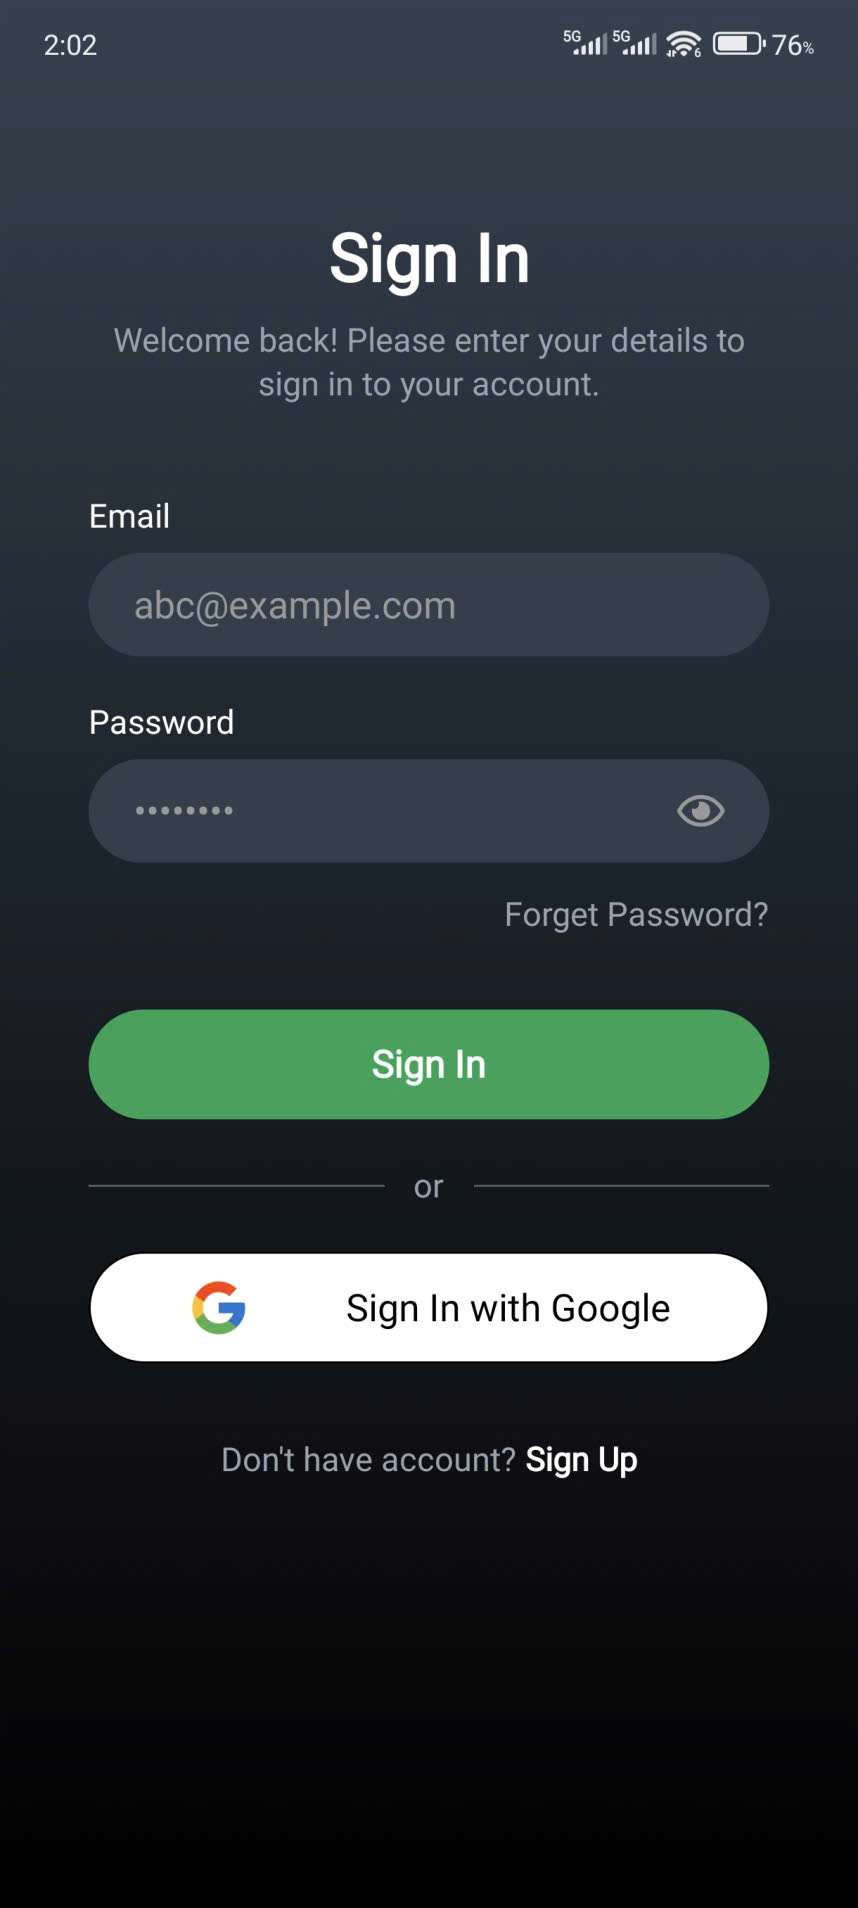
\includegraphics[width=\linewidth]{figures/mobileScreen/signin.jpg}
        \caption*{Đăng nhập}
    \end{subfigure}
    \hfill
    \begin{subfigure}{0.32\linewidth}
        \centering
        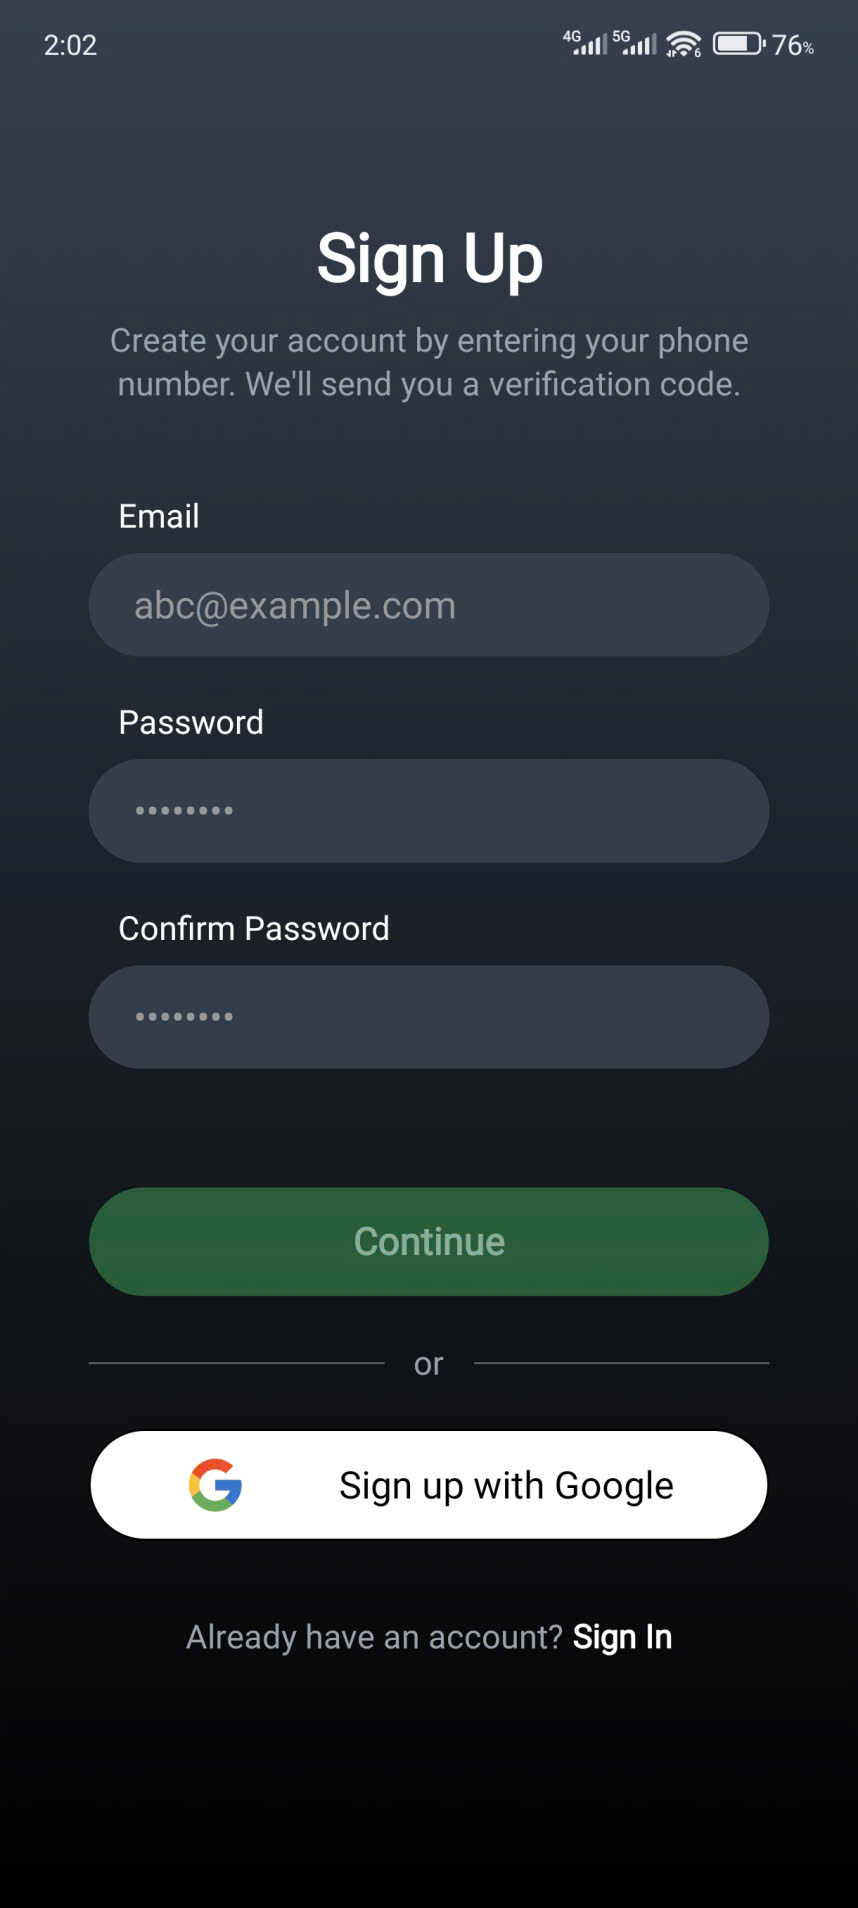
\includegraphics[width=\linewidth]{figures/mobileScreen/signup.jpg}
        \caption*{Đăng ký}
    \end{subfigure}
    \hfill
    \begin{subfigure}{0.32\linewidth}
        \centering
        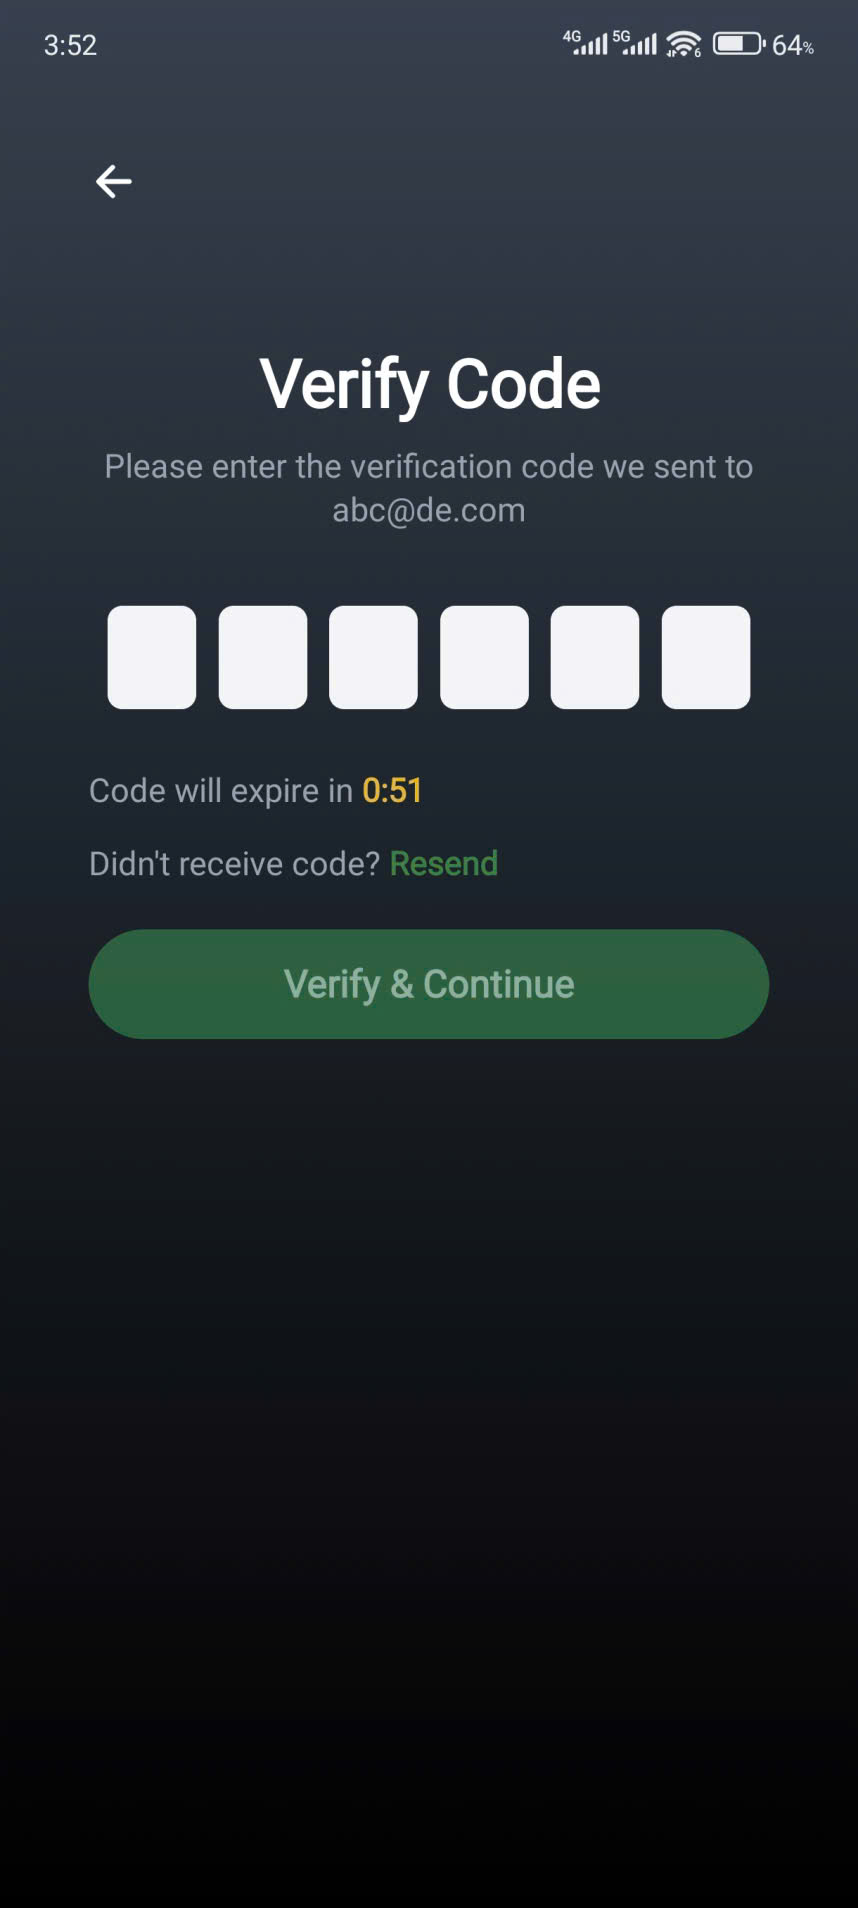
\includegraphics[width=\linewidth]{figures/mobileScreen/verifyOtp.jpg}
        \caption*{Xác thực OTP}
    \end{subfigure}

    \caption{Các màn hình xác thực tài khoản}
    \label{fig:auth-screens1}
\end{figure}

\subsubsection{Giao diện quản lý thông tin}
Giao diện gồm các màn hình chính để người dùng quản lý thông tin cá nhân và danh sách phương tiện
\begin{figure}[H]
    \centering
    \begin{subfigure}{0.32\linewidth}
        \centering
        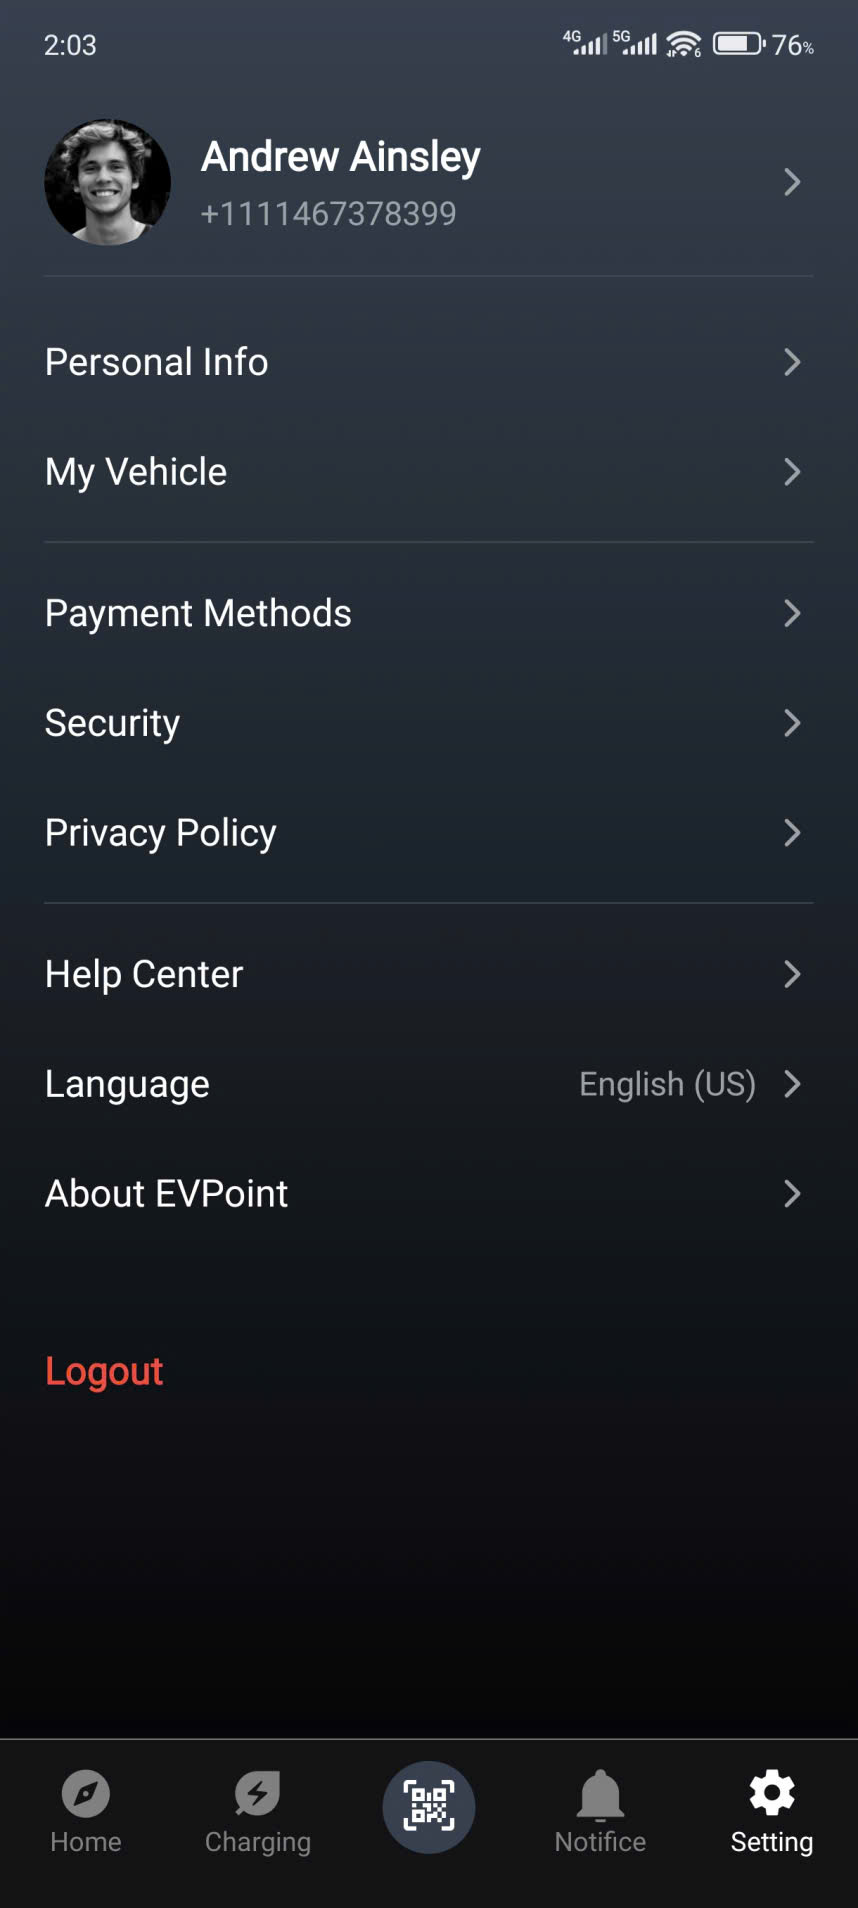
\includegraphics[width=\linewidth]{figures/mobileScreen/setting.jpg}
        \caption*{Cài đặt}
    \end{subfigure}
    \hfill
    \begin{subfigure}{0.32\linewidth}
        \centering
        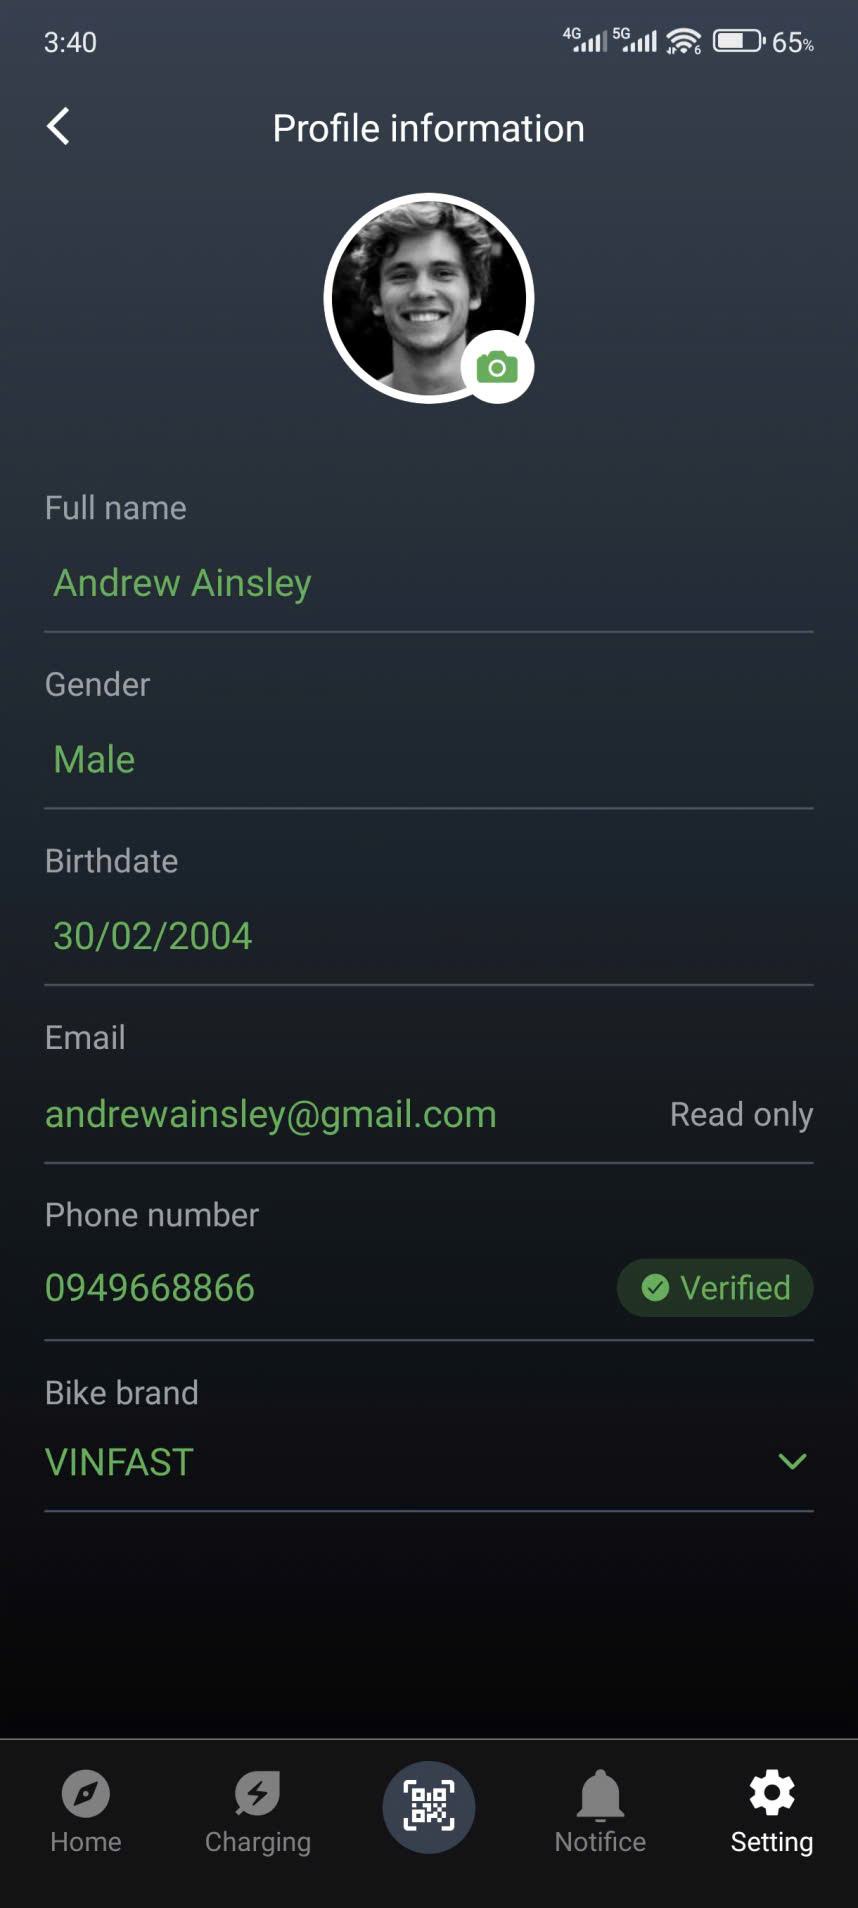
\includegraphics[width=\linewidth]{figures/mobileScreen/profile.jpg}
        \caption*{Thông tin cá nhân}
    \end{subfigure}
    \hfill
    \begin{subfigure}{0.32\linewidth}
        \centering
        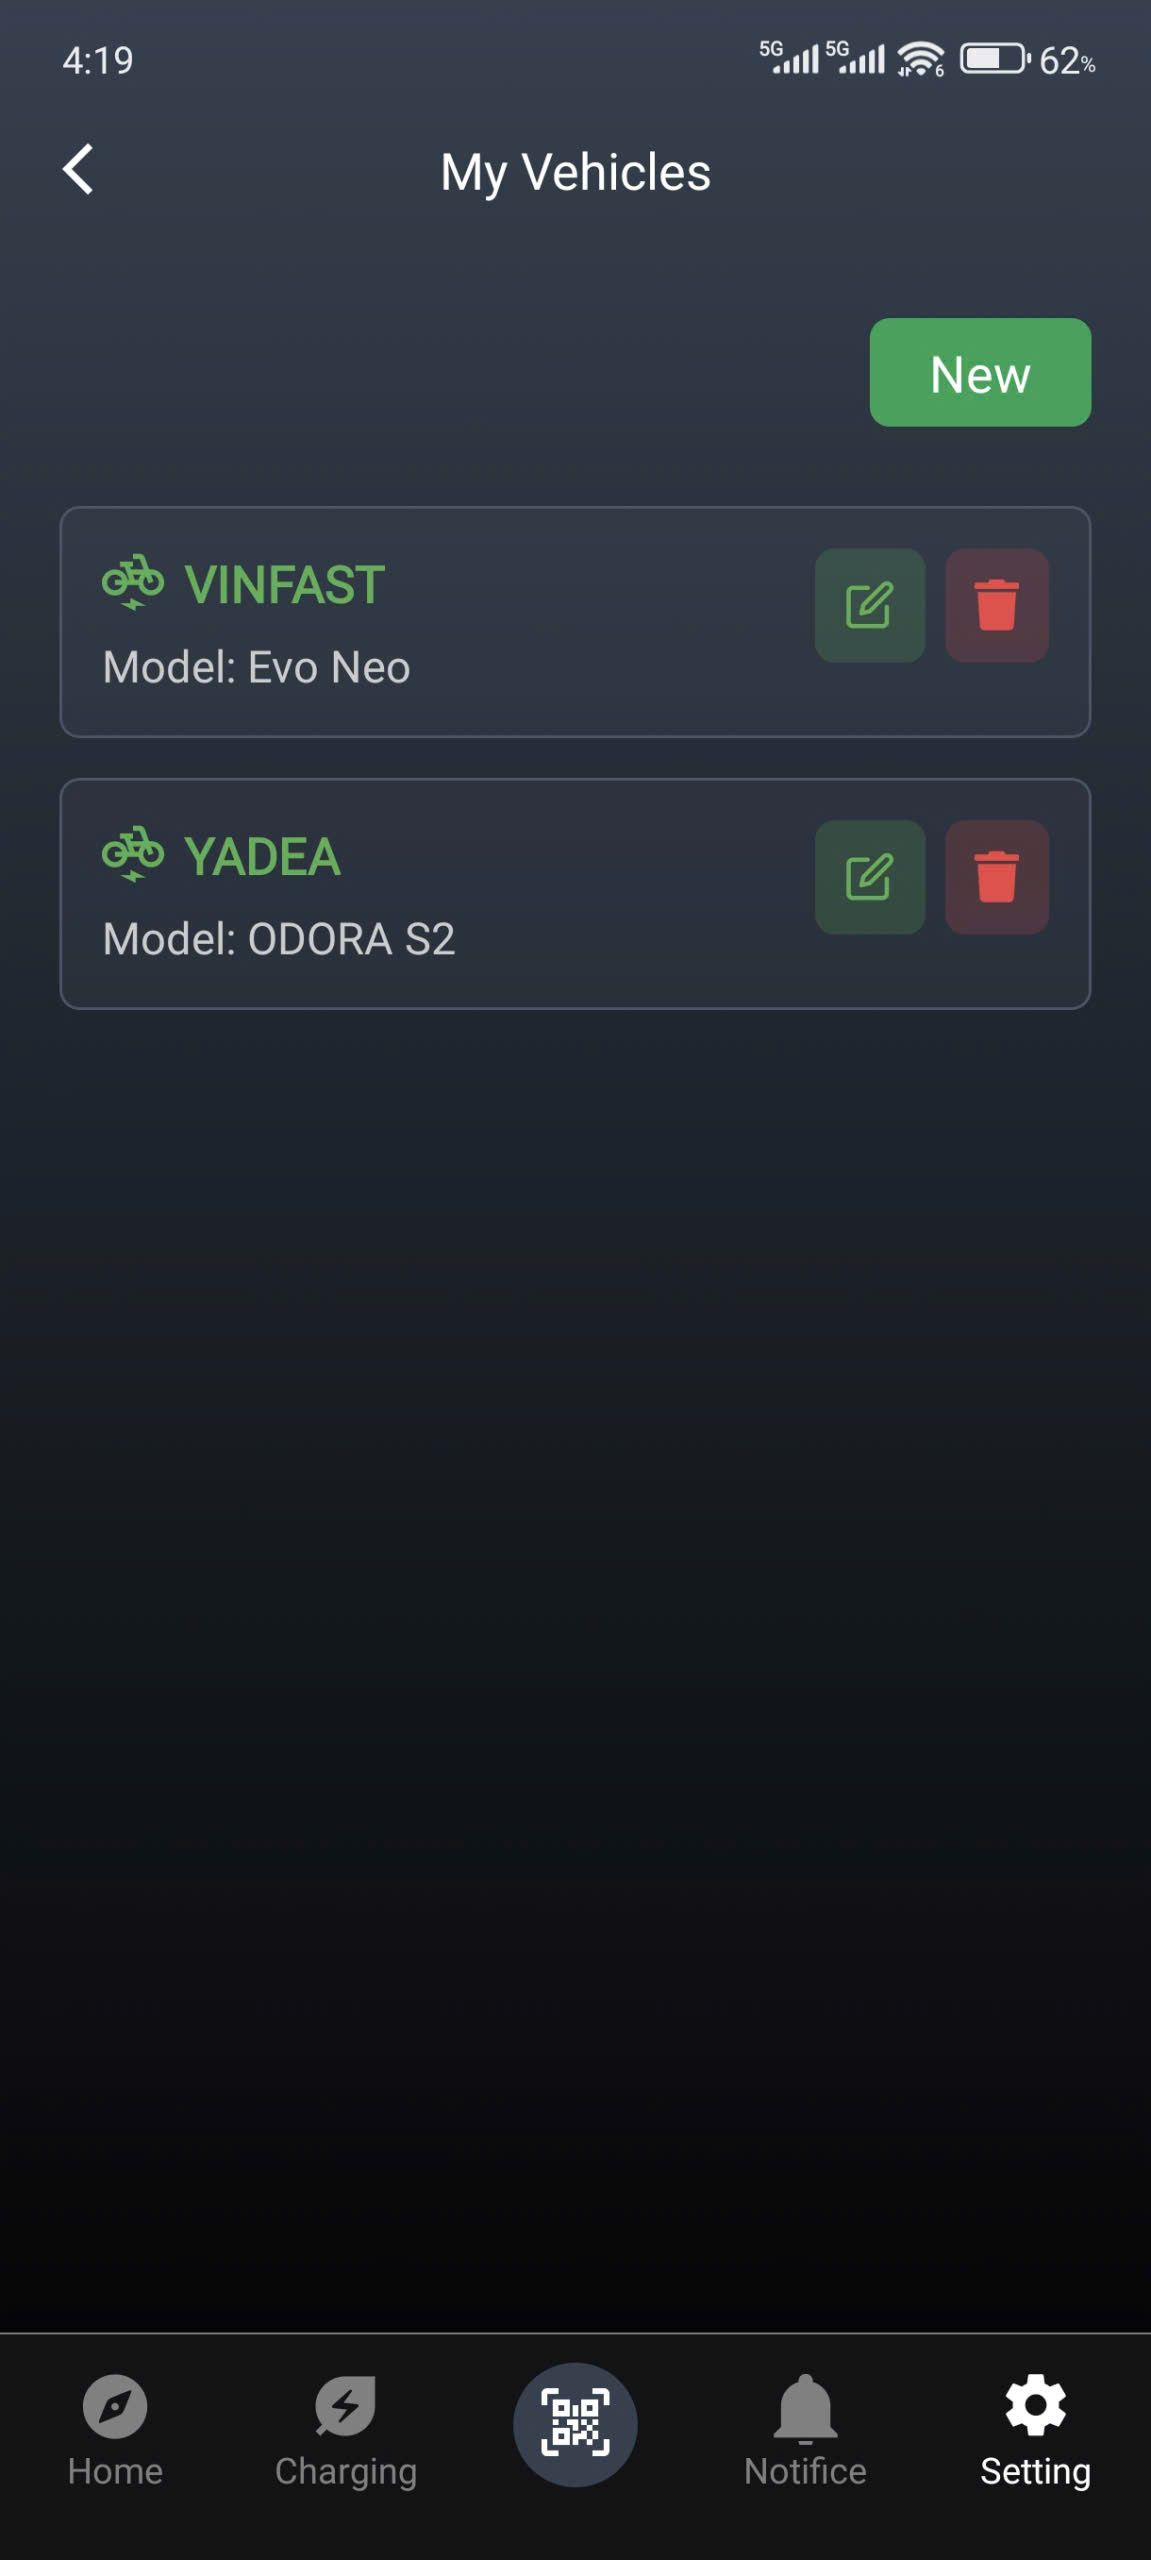
\includegraphics[width=\linewidth]{figures/mobileScreen/myVehicle.jpg}
        \caption*{Quản lý phương tiện}
    \end{subfigure}

    \caption{Các màn hình quản lý thông tin}
    \label{fig:auth-screens2}
\end{figure}

\subsection{Giao diện website}

\newpage
% ============================================================
%  Chương 7 — Kiểm thử và Đánh giá
% ============================================================
\section{Kiểm thử và Đánh giá}

% ------------------------------------------------------------
\subsection{Chiến lược kiểm thử}
% ------------------------------------------------------------
\hspace*{\parindent}
Đảm bảo chất lượng phần mềm là yếu tố then chốt trong vòng đời phát triển
hệ thống EVGo. Với đặc thù là nền tảng quản lý trạm sạc xe máy điện có các giao dịch
thời gian thực, bất kỳ sai sót nào trong luồng đặt chỗ, sạc điện hay thanh toán
đều có thể gây ra tổn thất nghiêm trọng cho người dùng và đối tác vận hành.

Nhóm áp dụng chiến lược kiểm thử theo ba tầng độc lập nhưng bổ trợ lẫn nhau:

\begin{itemize}
    \item \textbf{Unit Testing:} Tập trung xác minh tính đúng đắn của các khối logic nghiệp vụ lõi tại tầng Dịch vụ (Service) và các bộ lắng nghe sự kiện (Event Listener). Quá trình này được thực hiện trong môi trường hoàn toàn cô lập, tách biệt độc lập khỏi các phụ thuộc vào cơ sở hạ tầng bên ngoài.

    \item \textbf{Manual \& End-to-End Testing:} Đánh giá toàn diện luồng nghiệp vụ từ phía ứng dụng người dùng (Frontend) đến hệ thống xử lý trung tâm (Backend). Quá trình này được thực hiện trên giao diện ứng dụng thực tế, kết hợp sử dụng công cụ giả lập OCPP ChargePoint Simulator để mô phỏng chính xác các tương tác vật lý với hệ thống trụ sạc.

    \item \textbf{Performance Testing:} Đánh giá độ ổn định và khả năng đáp ứng của hệ thống dưới áp lực truy cập đồng thời quy mô lớn. Các kịch bản chịu tải được mô phỏng và đo lường chi tiết thông qua bộ công cụ Apache JMeter~\cite{jmeter}.
\end{itemize}

% ------------------------------------------------------------
\subsection{Unit Testing}
% ------------------------------------------------------------

\subsubsection{Mục tiêu và bộ công cụ}

\hspace*{\parindent}
Trọng tâm của giai đoạn Unit Testing là xây dựng một bộ kịch bản kiểm thử
toàn diện nhằm bảo vệ an toàn luồng dữ liệu cho các module cốt lõi của Backend.
Các module được ưu tiên hàng đầu bao gồm: \textit{Station}, \textit{Booking},
\textit{Charging}, \textit{Payment} và \textit{OCPP}. Nhóm bám sát hai chỉ tiêu
chất lượng cụ thể:

\begin{itemize}
    \item \textbf{Độ phủ kịch bản:} Hoàn thành \textbf{100\%} các kịch bản chuẩn và kịch bản sinh lỗi.

    \item \textbf{Độ phủ mã lệnh:} Duy trì tỷ lệ tối thiểu \textbf{80\%} đối với các lớp chứa logic nghiệp vụ.
\end{itemize}

Để đạt được các chỉ tiêu này, nhóm sử dụng bộ công cụ tiêu chuẩn của hệ sinh thái
Spring Boot:

\begin{itemize}
    \item \textbf{JUnit 5}~\cite{junit5}: Đóng vai trò là Test Runner chính.
          Tên các phương thức kiểm thử được viết theo quy ước thống nhất.

    \item \textbf{Mockito}~\cite{mockito}: Sử dụng \texttt{@Mock} và
          \texttt{@InjectMocks} để giả lập các thành phần phụ thuộc. Việc này giúp cô lập môi trường kiểm thử khỏi cơ sở hạ tầng thực. Hàm \texttt{verify()} được áp dụng để kiểm chứng tính chính xác của tương tác giữa các thành phần.

    \item \textbf{AssertJ}~\cite{assertj}: Sử dụng Fluent API để các câu lệnh kiểm chứng đọc tự nhiên và dễ gỡ lỗi, đặc biệt khi cần bắt và đối chiếu mã lỗi chuẩn.

    \item \textbf{JaCoCo 0.8.11}~\cite{jacoco}: Tích hợp trực tiếp vào pipeline
          Maven để đo lường và báo cáo độ phủ mã nguồn sau mỗi lần chạy kiểm thử.
\end{itemize}

% ------------------------------------------------------------
\subsubsection{Quy trình phát triển hướng kiểm thử}

\hspace*{\parindent}
Toàn bộ các tính năng mới đều được phát triển theo vòng lặp
\textbf{Phát triển Hướng Kiểm thử (TDD)} gồm ba bước cốt lõi:

\begin{enumerate}
    \item \textbf{Viết kiểm thử trước:} Dựa trên tài liệu thiết kế nghiệp vụ, nhóm chủ động soạn thảo các kịch bản kiểm thử bao phủ cả luồng chuẩn và luồng sinh lỗi. Ở giai đoạn này, toàn bộ kịch bản kiểm thử đều chạy thất bại do logic chưa được cài đặt.

    \item \textbf{Hiện thực logic tối giản:} Nhóm triển khai phần logic cốt lõi với khối lượng mã nguồn gọn nhẹ nhưng đủ để toàn bộ kịch bản kiểm thử chuyển sang trạng thái thành công.

    \item \textbf{Tái cấu trúc và gia cố:} Tối ưu, làm sạch mã nguồn trong khi vẫn duy trì tỷ lệ vượt qua 100\%. Đây cũng là thời điểm nhóm bổ sung các trường hợp ngoại lệ như yêu cầu rỗng, định danh giả mạo, hay xung đột dữ liệu đồng thời.
\end{enumerate}

Mỗi kịch bản kiểm thử đều được cấu trúc theo mẫu \textbf{Given -- When -- Then},
phân tách thành ba khối rõ ràng nhằm tăng khả năng đọc hiểu và bảo trì:

\begin{itemize}
    \item \textbf{Given:} Thiết lập ngữ cảnh, chuẩn bị dữ liệu giả lập và các điều kiện đầu vào.
    \item \textbf{When:} Gọi thực thi phương thức cần kiểm thử.
    \item \textbf{Then:} Kiểm định đầu ra, đối chiếu kết quả thực tế với kỳ vọng thiết kế.
\end{itemize}

% ------------------------------------------------------------
\subsubsection{Kết quả Unit Testing}

\hspace*{\parindent}
Bộ kiểm thử của hệ thống EVGo bao gồm tổng cộng \textbf{37 lớp kiểm thử}
phân bổ trên 8 module chức năng, với \textbf{334 kịch bản kiểm thử} được thực thi.
Kết quả cho thấy toàn bộ kịch bản đều vượt qua thành công mà không ghi nhận bất kỳ
lỗi hay ngoại lệ nào.

\begin{figure}[H]
    \centering
    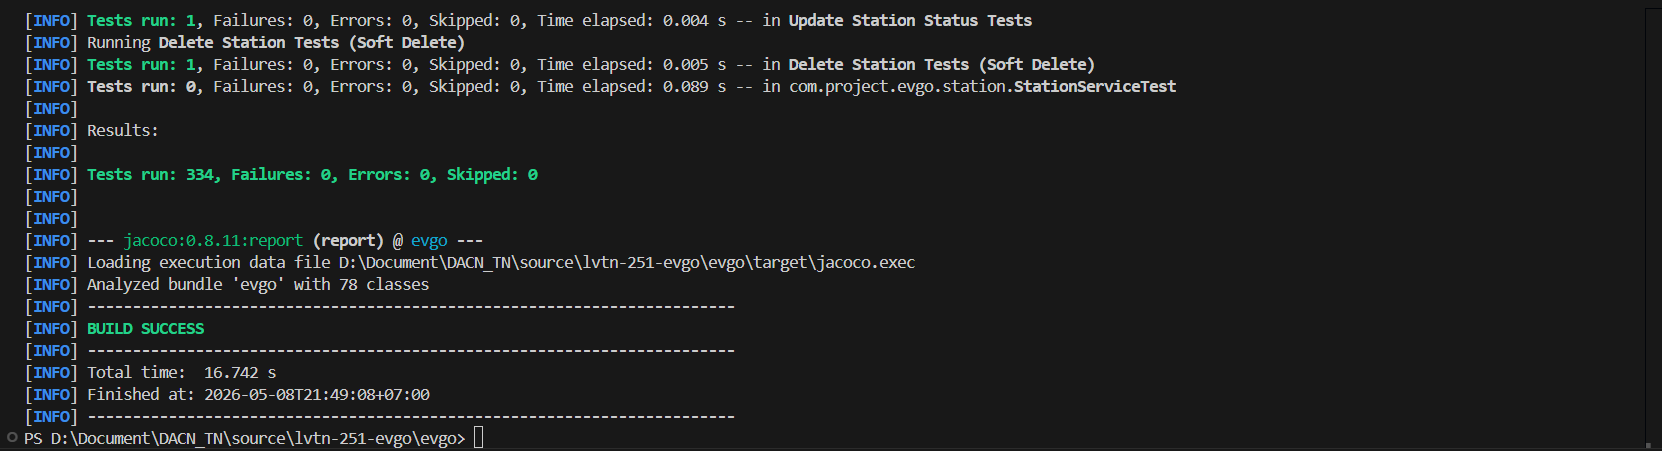
\includegraphics[width=\textwidth]{figures/test/unitTest.png}
    \caption{Kết quả chạy toàn bộ bộ unit test qua Maven
             (334 tests run, 0 failures, 0 errors, 0 skipped)}
    \label{fig:unit_test_result}
\end{figure}

Bảng~\ref{tab:unit_test_summary} trình bày phân bổ số lượng kịch bản kiểm thử
theo từng module chức năng:

\begin{center}
    \renewcommand{\arraystretch}{1.5}
    \begin{longtable}{|>{\raggedright\arraybackslash}m{0.15\textwidth}|>{\raggedright\arraybackslash}m{0.5\textwidth}|c|c|}
        \caption{Tổng hợp kịch bản unit test theo module}
        \label{tab:unit_test_summary} \\
        \hline
        \textbf{Module} & \textbf{Lớp kiểm thử tiêu biểu} & \textbf{Số lớp} & \textbf{Số kịch bản} \\
        \hline
        \endfirsthead
        
        \hline
        \textbf{Module} & \textbf{Lớp kiểm thử tiêu biểu} & \textbf{Số lớp} & \textbf{Số kịch bản} \\
        \hline
        \endhead
        
        Station   & StationServiceTest, StationAdminServiceImplTest, StationPhotoServiceTest, PriceSettingServiceTest & 6 & 87 \\
        \hline
        Booking   & BookingServiceTest, BookingEventListenerTest, BookingSchedulerTest & 6 & 43 \\
        \hline
        Charging  & ChargingServiceTest, ChargingMonitorServiceTest, OcppChargingEventListenerTest & 3 & 40 \\
        \hline
        OCPP      & OcppMessageParserTest, OcppWebSocketHandlerTest, MeterValuesHandlerTest, StatusNotificationHandlerTest & 7 & 53 \\
        \hline
        Payment   & InvoiceServiceImplTest, ZaloPayServiceTest, ChargingInvoiceListenerTest, IdleFeeListenerTest & 5 & 36 \\
        \hline
        Notification & PushNotificationEventListenerTest, PushTokenServiceTest, SmtpEmailServiceImplTest & 3 & 17 \\
        \hline
        Review    & ReviewServiceTest, ReviewDtoConverterTest & 2 & 20 \\
        \hline
        Hạ tầng   & ModularityTests, DocumenterTests, EvgoApplicationTests & 3 & 3 \\
        \hline
        \multicolumn{2}{|r|}{\textbf{Tổng}} & \textbf{37} & \textbf{334} \\
        \hline
    \end{longtable}
\end{center}

% ------------------------------------------------------------
\subsubsection{Độ phủ mã nguồn}

\hspace*{\parindent}
Sau khi toàn bộ bộ kiểm thử được thực thi, công cụ JaCoCo~\cite{jacoco} tự động
tổng hợp và trình bày báo cáo độ phủ mã nguồn theo từng package. Kết quả thu được
từ hình~\ref{fig:jacoco_overview} chứng minh hệ thống đã đạt và vượt ngưỡng chất
lượng đề ra:

\begin{figure}[H]
    \centering
    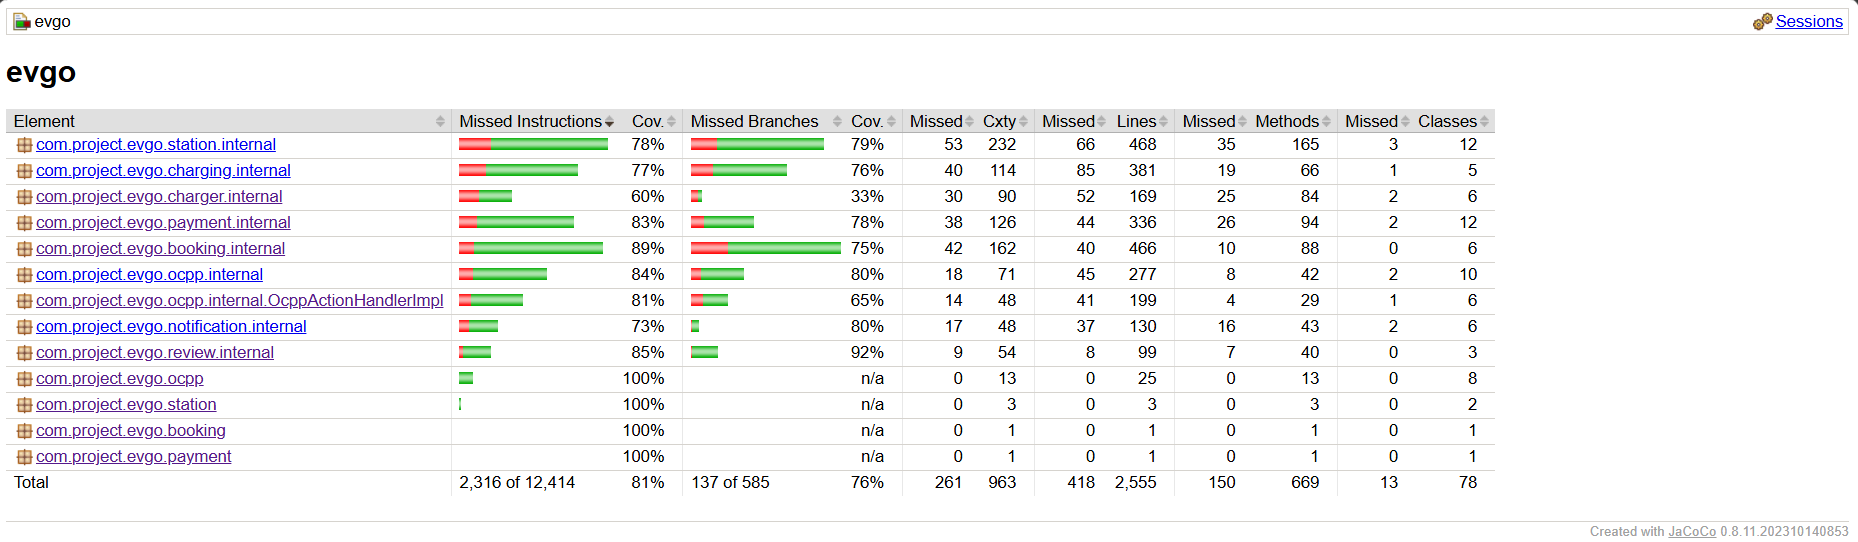
\includegraphics[width=\textwidth]{figures/test/coverage.png}
    \caption{Báo cáo độ phủ mã nguồn tổng thể theo JaCoCo 0.8.11}
    \label{fig:jacoco_overview}
\end{figure}

\begin{center}
    \renewcommand{\arraystretch}{1.5}
    \begin{longtable}{|>{\raggedright\arraybackslash}m{0.45\textwidth}|c|c|c|c|}
        \caption{Độ phủ mã nguồn theo từng package (JaCoCo)}
        \label{tab:jacoco_coverage} \\
        \hline
        \textbf{Package} & \textbf{Instr. Cov.} & \textbf{Branch Cov.} & \textbf{Lines} & \textbf{Methods} \\
        \hline
        \endfirsthead
        
        \hline
        \textbf{Package} & \textbf{Instr. Cov.} & \textbf{Branch Cov.} & \textbf{Lines} & \textbf{Methods} \\
        \hline
        \endhead
        
        com.project.evgo.booking.internal    & 89\% & 75\% & 466 & 88 \\
        \hline
        com.project.evgo.station.internal    & 78\% & 79\% & 468 & 165 \\
        \hline
        com.project.evgo.payment.internal    & 83\% & 78\% & 336 & 94 \\
        \hline
        com.project.evgo.charging.internal   & 77\% & 76\% & 381 & 66 \\
        \hline
        com.project.evgo.ocpp.internal       & 84\% & 80\% & 277 & 42 \\
        \hline
        com.project.evgo.review.internal     & 85\% & 92\% & 99  & 40 \\
        \hline
        com.project.evgo.notification.internal & 73\% & 80\% & 130 & 43 \\
        \hline
        com.project.evgo.charger.internal    & 60\% & 33\% & 169 & 84 \\
        \hline
        \textbf{Tổng hệ thống (78 classes)} & \textbf{81\%} & \textbf{76\%} & \textbf{2.555} & \textbf{669} \\
        \hline
    \end{longtable}
\end{center}

Phân tích chi tiết các chỉ số cho thấy:

\begin{itemize}
    \item \textbf{Độ phủ tập lệnh (81\%):} Vượt ngưỡng mục tiêu 80\%, khẳng định phần lớn các tập lệnh trong luồng logic cốt lõi đã được thực thi và kiểm chứng.

    \item \textbf{Độ phủ rẽ nhánh (76\%):} Đảm bảo các luồng rẽ nhánh quan trọng đã được bao phủ, giúp giảm thiểu rủi ro phát sinh lỗi logic tại các tình huống biên.

    \item \textbf{Module booking.internal (89\% / 75\%):} Đạt mức phủ cao nhất về tập lệnh, phản ánh mức độ ưu tiên kiểm thử đối với luồng nghiệp vụ phức tạp nhất của hệ thống, bao gồm cơ chế khoá phân tán trên Redis và phát các sự kiện nội bộ.

    \item \textbf{Module charger.internal (60\% / 33\%):} Ghi nhận mức phủ thấp hơn do phần lớn các lớp trong module này đóng vai trò là các đối tượng giao tiếp và cầu nối dữ liệu, không chứa logic nghiệp vụ phức tạp.
\end{itemize}

% ------------------------------------------------------------
\subsection{Manual \& End-to-End Testing}
% ------------------------------------------------------------

\hspace*{\parindent}
Đối với các tính năng cần thực hiện giao tiếp với trụ sạc theo đúng chuẩn OCPP 1.6J, nhóm sử dụng công cụ giả lập OCPP ChargePoint Simulator để đóng vai trò làm phần cứng trụ sạc.

\subsubsection{Chuẩn bị môi trường mô phỏng}

\begin{enumerate}
    \item Mở trang Web giả lập trạm sạc: \url{https://shiv3.github.io/ocpp-cp-simulator/}.
    \item Tại trường \textbf{Central System URL}, nhập địa chỉ WebSocket của Backend đang chạy, ví dụ: \texttt{ws://localhost:8081/ocpp/}.
    \item Tại trường \textbf{Charge Point Identity}, nhập ID của trụ sạc có trong cơ sở dữ liệu. Tại trường \textbf{Number of Connectors}, nhập số lượng cổng của trụ. Sau khi cấu hình xong, nhấn lưu lại để tạo bản mô phỏng.
    
    \begin{figure}[H]
        \centering
        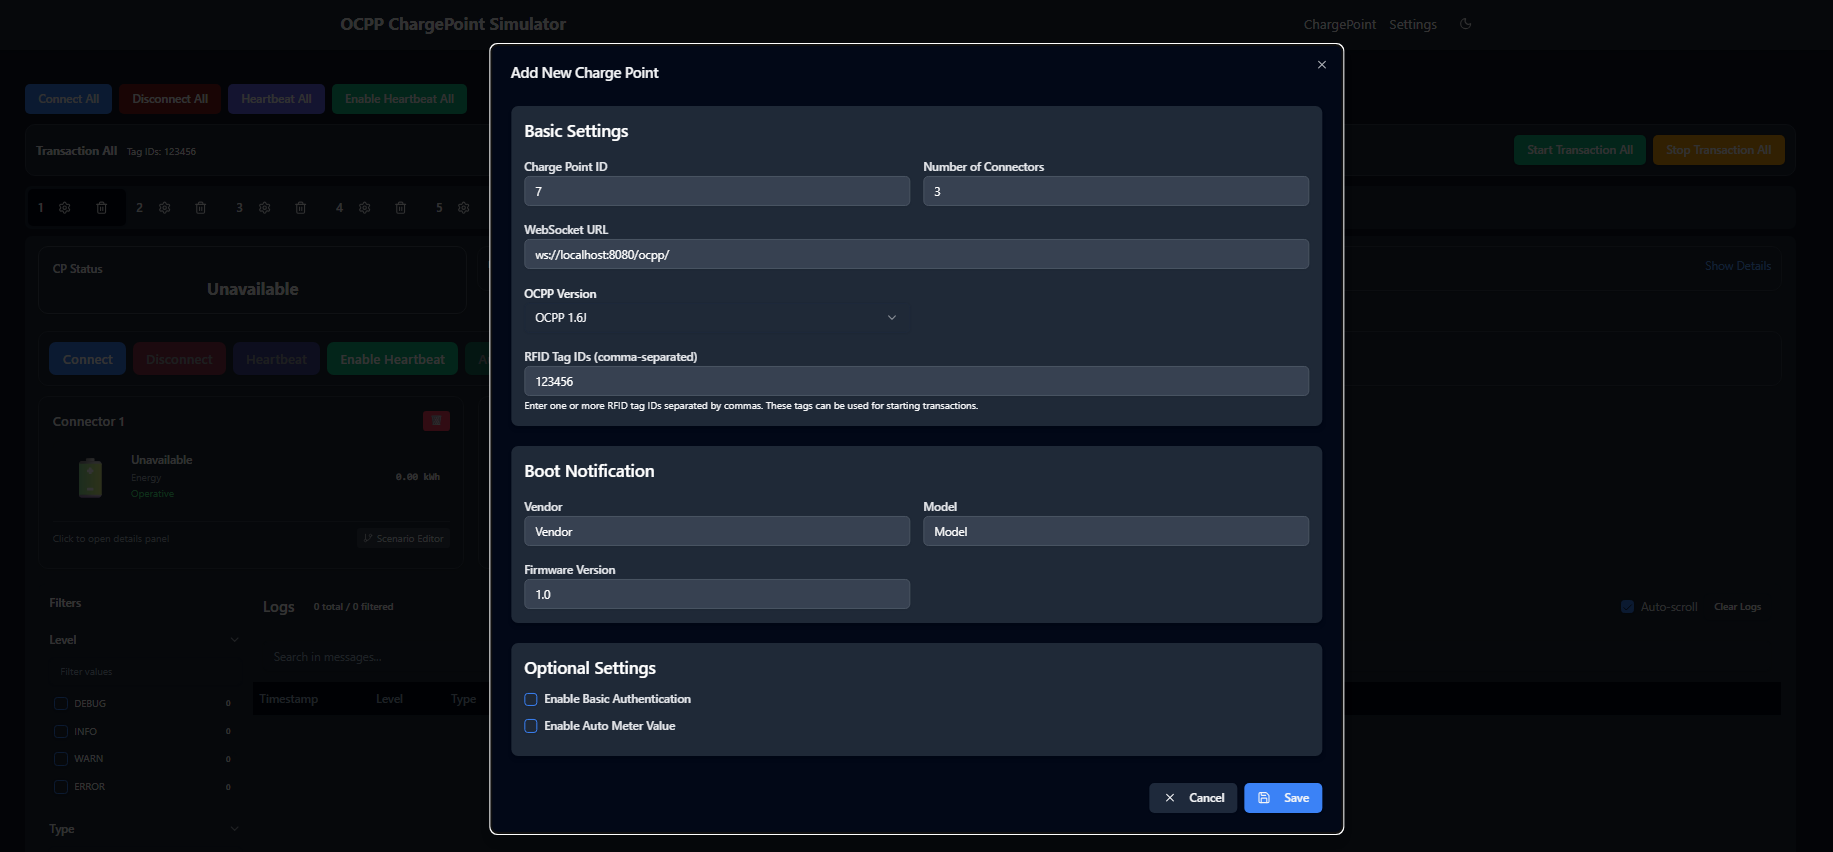
\includegraphics[width=0.9\textwidth]{figures/test/ocppWeb.png}
        \caption{Giao diện cấu hình và khởi tạo bản mô phỏng trụ sạc}
        \label{fig:ocpp_web_setup}
    \end{figure}

    \item Bấm nút \textbf{Connect}, sau đó quan sát Backend log báo đã nhận được sự kiện \texttt{BootNotification}. Lúc này, quá trình kết nối với trụ sạc đã thành công và hệ thống đã sẵn sàng để thực hiện các luồng kiểm thử liên quan tới phần cứng.
    
    \begin{figure}[H]
        \centering
        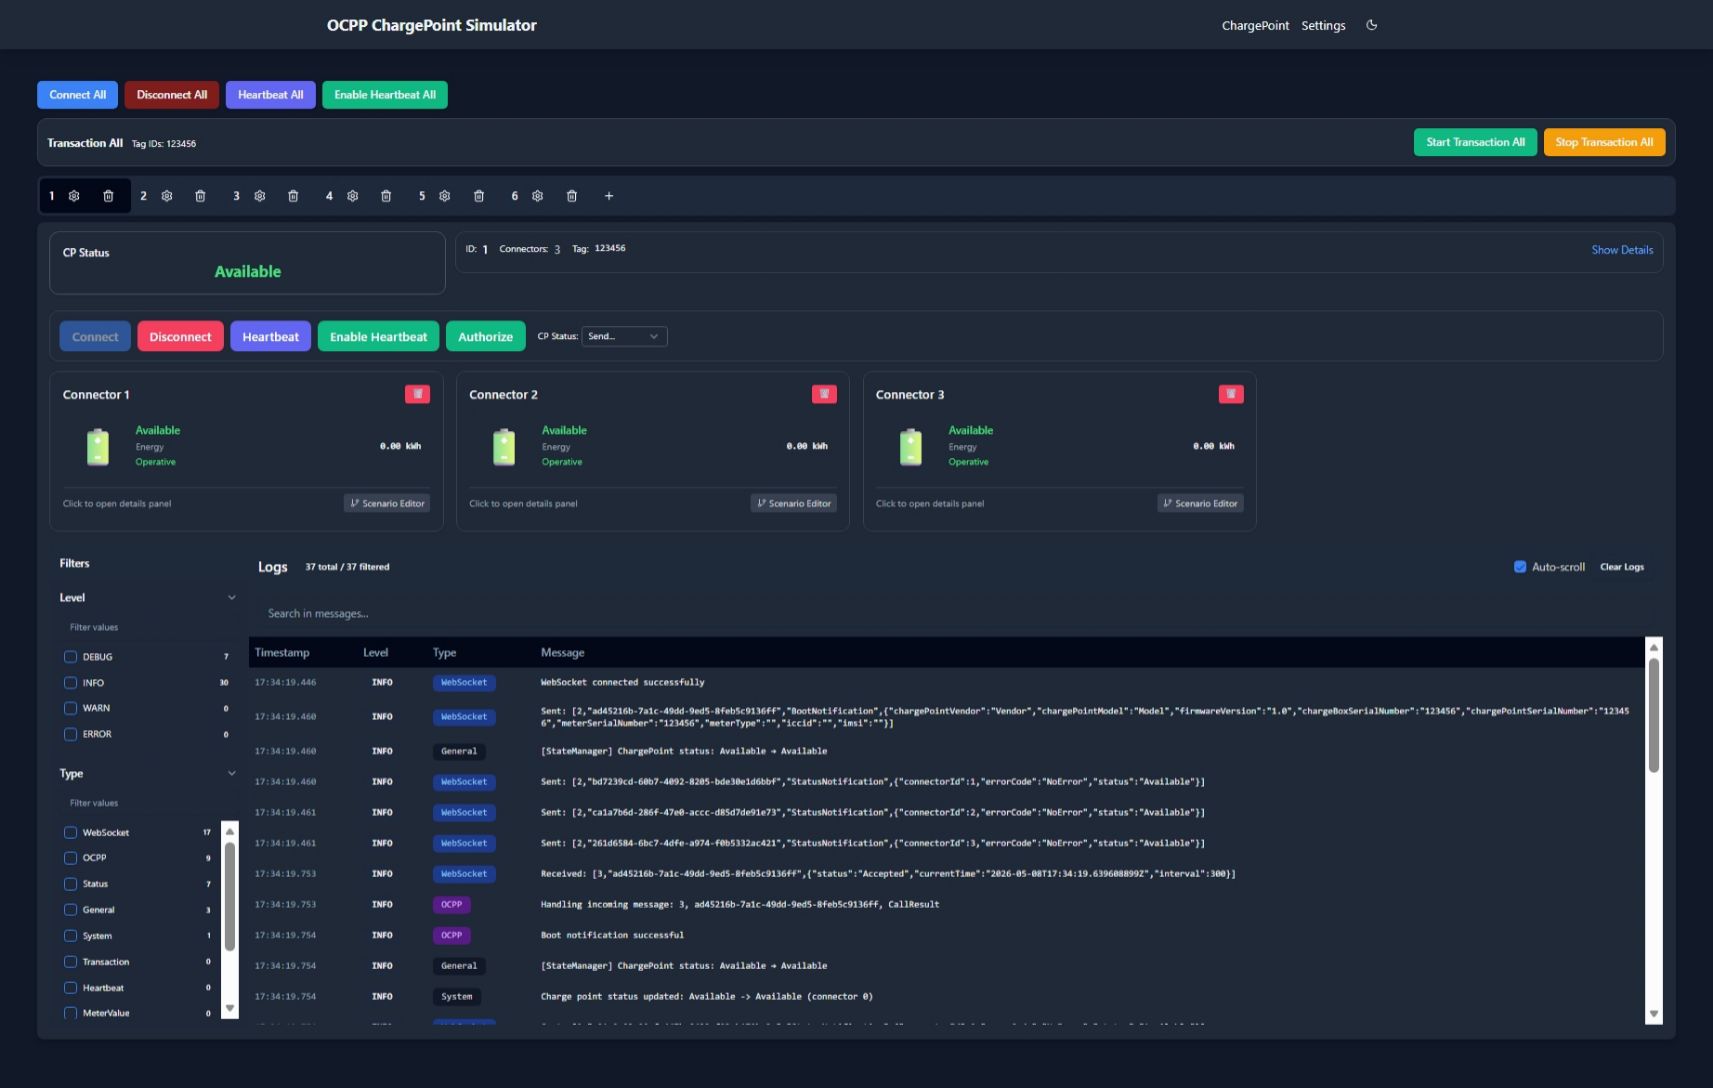
\includegraphics[width=0.9\textwidth]{figures/test/ocppConnect.png}
        \caption{Trụ sạc mô phỏng kết nối thành công với Backend qua WebSocket}
        \label{fig:ocpp_connect}
    \end{figure}
\end{enumerate}

Dưới đây là tổng hợp các kịch bản kiểm thử thủ công cho từng nhóm chức năng trọng yếu:

\subsubsection{Nhóm chức năng: Bản đồ trạm sạc}

\begin{center}
    \renewcommand{\arraystretch}{1.5}
    \begin{longtable}{|c|>{\raggedright\arraybackslash}m{0.25\textwidth}|>{\raggedright\arraybackslash}m{0.3\textwidth}|>{\raggedright\arraybackslash}m{0.3\textwidth}|}
        \caption{Kịch bản kiểm thử luồng chuẩn - Bản đồ trạm sạc}
        \label{tab:map_happy} \\
        \hline
        \textbf{Bước} & \textbf{Hành động} & \textbf{Kết quả kỳ vọng} & \textbf{Kết quả thực tế} \\
        \hline
        \endfirsthead
        
        \hline
        \textbf{Bước} & \textbf{Hành động} & \textbf{Kết quả kỳ vọng} & \textbf{Kết quả thực tế} \\
        \hline
        \endhead
        
        1 & Mở màn hình bản đồ. & Tự động lấy vị trí hiện tại của người dùng; Hiển thị các biểu tượng trạm sạc xung quanh. & Khớp. Bản đồ tải mượt, các biểu tượng hiển thị đúng vị trí trong cơ sở dữ liệu. \\
        \hline
        2 & Sử dụng bộ lọc (Filter) theo loại trụ sạc hoặc trạng thái. & Bản đồ chỉ hiển thị các trạm sạc thỏa mãn điều kiện lọc. & Khớp. API filterStations trả về đúng danh sách. Biểu tượng trạm không phù hợp tự ẩn đi. \\
        \hline
        3 & Nhấn vào một biểu tượng trạm sạc trên bản đồ. & Hiển thị thông tin nhanh (Mini card): Tên trạm, khoảng cách, số lượng trụ trống. & Khớp. Hiển thị đúng thông tin trạm sạc đó từ cơ sở dữ liệu. \\
        \hline
        4 & Tìm kiếm trạm sạc theo tên địa danh/địa chỉ. & Bản đồ di chuyển đến vị trí tìm kiếm và hiển thị trạm sạc gần đó. & Khớp. Tích hợp Map API tìm kiếm địa điểm chính xác. \\
        \hline
    \end{longtable}
\end{center}

\begin{center}
    \renewcommand{\arraystretch}{1.5}
    \begin{longtable}{|>{\raggedright\arraybackslash}m{0.2\textwidth}|>{\raggedright\arraybackslash}m{0.25\textwidth}|>{\raggedright\arraybackslash}m{0.25\textwidth}|>{\raggedright\arraybackslash}m{0.2\textwidth}|}
        \caption{Kịch bản kiểm thử ngoại lệ - Bản đồ trạm sạc}
        \label{tab:map_negative} \\
        \hline
        \textbf{Tình huống} & \textbf{Hành động} & \textbf{Kết quả kỳ vọng} & \textbf{Kết quả thực tế} \\
        \hline
        \endfirsthead
        
        \hline
        \textbf{Tình huống} & \textbf{Hành động} & \textbf{Kết quả kỳ vọng} & \textbf{Kết quả thực tế} \\
        \hline
        \endhead
        
        Quyền vị trí & Người dùng từ chối cấp quyền truy cập vị trí (GPS). & Ứng dụng hiển thị thông báo yêu cầu cấp quyền hoặc cho phép nhập vị trí thủ công. & Đạt. Ứng dụng không bị lỗi, hiển thị một vị trí mặc định tại trung tâm TP.HCM. \\
        \hline
        Vùng không có trạm & Di chuyển bản đồ đến một vùng không có trạm sạc nào. & Ứng dụng hiển thị đúng trạng thái không có trạm sạc nào ở khu vực này. & Đạt. Xử lý tốt trường hợp danh sách trả về từ API bị rỗng. \\
        \hline
        Dẫn đường (Navigate) & Nhấn nút dẫn đường đến trạm. & Dẫn đường ngay trong ứng dụng, không bị dừng đột ngột. & Đạt. Ứng dụng xử lý luồng mượt mà, vị trí được cập nhật. \\
        \hline
    \end{longtable}
\end{center}

\subsubsection{Nhóm chức năng: Thanh toán}

\begin{center}
    \renewcommand{\arraystretch}{1.5}
    \begin{longtable}{|c|>{\raggedright\arraybackslash}m{0.25\textwidth}|>{\raggedright\arraybackslash}m{0.3\textwidth}|>{\raggedright\arraybackslash}m{0.3\textwidth}|}
        \caption{Kịch bản kiểm thử luồng chuẩn - Thanh toán}
        \label{tab:payment_happy} \\
        \hline
        \textbf{Bước} & \textbf{Hành động} & \textbf{Kết quả kỳ vọng} & \textbf{Kết quả thực tế} \\
        \hline
        \endfirsthead
        
        \hline
        \textbf{Bước} & \textbf{Hành động} & \textbf{Kết quả kỳ vọng} & \textbf{Kết quả thực tế} \\
        \hline
        \endhead
        
        1 & Chọn trụ sạc, thời gian và nhấn Thanh toán. & Ứng dụng hiển thị đúng số tiền tính toán. Chuyển sang ví ZaloPay. & Đạt. Ứng dụng hiển thị đúng số tiền tính toán. Chuyển trang sang ZaloPay Sandbox thành công. \\
        \hline
        2 & Xác nhận thanh toán trên App ZaloPay. & ZaloPay báo giao dịch thành công. & Đạt. Giao dịch được xác nhận trên môi trường Sandbox. \\
        \hline
        3 & Chờ hệ thống xử lý Callback. & Ứng dụng tự động cập nhật trạng thái Thành công. & Đạt. Màn hình tự cập nhật sau khoảng 2 giây. Trạng thái cơ sở dữ liệu chuyển sang PAID. \\
        \hline
        4 & Xem lại hóa đơn thanh toán. & Hóa đơn hiển thị đầy đủ thông tin. & Đạt. \\
        \hline
    \end{longtable}
\end{center}

\begin{center}
    \renewcommand{\arraystretch}{1.5}
    \begin{longtable}{|>{\raggedright\arraybackslash}m{0.2\textwidth}|>{\raggedright\arraybackslash}m{0.25\textwidth}|>{\raggedright\arraybackslash}m{0.25\textwidth}|>{\raggedright\arraybackslash}m{0.2\textwidth}|}
        \caption{Kịch bản kiểm thử ngoại lệ - Thanh toán}
        \label{tab:payment_negative} \\
        \hline
        \textbf{Tình huống} & \textbf{Hành động} & \textbf{Kết quả kỳ vọng} & \textbf{Kết quả thực tế} \\
        \hline
        \endfirsthead
        
        \hline
        \textbf{Tình huống} & \textbf{Hành động} & \textbf{Kết quả kỳ vọng} & \textbf{Kết quả thực tế} \\
        \hline
        \endhead
        
        Hủy giao dịch & Nhấn hủy trên ví ZaloPay. & Ứng dụng thông báo giao dịch chưa được thực hiện và chờ thử lại. & Đạt. \\
        \hline
        Giả mạo dữ liệu & Gửi Callback giả bằng Postman với chữ ký (Signature) sai. & Hệ thống từ chối cập nhật và trả về mã lỗi 400. & Đạt. Hệ thống log lỗi chữ ký không hợp lệ, không có dữ liệu nào bị thay đổi trái phép. \\
        \hline
        Thanh toán trùng & Nhấn nút thanh toán nhiều lần liên tiếp. & Chỉ có duy nhất một giao dịch được tạo ra trên ZaloPay. & Đạt. Cơ chế Idempotency xử lý tốt, không tạo trùng đơn hàng trong cơ sở dữ liệu. \\
        \hline
    \end{longtable}
\end{center}

\subsubsection{Nhóm chức năng: Đặt chỗ}

\begin{center}
    \renewcommand{\arraystretch}{1.5}
    \begin{longtable}{|c|>{\raggedright\arraybackslash}m{0.25\textwidth}|>{\raggedright\arraybackslash}m{0.3\textwidth}|>{\raggedright\arraybackslash}m{0.3\textwidth}|}
        \caption{Kịch bản kiểm thử luồng chuẩn - Đặt chỗ}
        \label{tab:booking_happy} \\
        \hline
        \textbf{Bước} & \textbf{Hành động} & \textbf{Kết quả kỳ vọng} & \textbf{Kết quả thực tế} \\
        \hline
        \endfirsthead
        
        \hline
        \textbf{Bước} & \textbf{Hành động} & \textbf{Kết quả kỳ vọng} & \textbf{Kết quả thực tế} \\
        \hline
        \endhead
        
        1 & Trên ứng dụng, người dùng chọn một trạm sạc, chọn trụ sạc, chọn cổng sạc và chọn khung giờ bắt đầu và kết thúc. & Hệ thống kiểm tra không có đặt chỗ nào trùng lặp. Hệ thống tạo các khóa phân tán trên Redis (Atomic Lock) để giữ chỗ tạm thời cho người dùng hiện tại. & Khớp. Cổng sạc được giữ chỗ tạm trên Redis cho đúng người dùng hiện tại, người khác không thể chọn trùng khung giờ. \\
        \hline
        2 & Người dùng xác nhận thông tin và nhấn Đặt chỗ. & Ứng dụng xác minh lại khóa Redis còn thuộc về người dùng hiện tại, tính phí đặt chỗ dựa trên bảng giá, lưu yêu cầu với trạng thái PENDING và tự động sinh hóa đơn cọc. & Khớp. Yêu cầu được tạo với trạng thái PENDING. Hóa đơn tương ứng được tạo và sẵn sàng thanh toán ZaloPay. \\
        \hline
        3 & Người dùng nhấn thanh toán và hoàn tất thanh toán bằng ZaloPay. & Hệ thống nhận sự kiện thanh toán thành công, cập nhật trạng thái sang CONFIRMED, xóa toàn bộ khóa Redis liên quan. Nếu khung giờ sạc gần hiện tại (trong 10 phút), tự động gửi lệnh ReserveNow đến trạm sạc vật lý. & Khớp. Đặt chỗ chuyển sang CONFIRMED, khóa Redis được giải phóng, gửi lệnh giữ chỗ thành công nếu khung giờ sát hiện tại. \\
        \hline
        4 & Người dùng mở danh sách lịch chờ sạc (My Bookings). & Trả về danh sách đặt chỗ đang chờ sạc của người dùng. & Khớp. Danh sách hiển thị đúng các đặt chỗ đã được xác nhận, kèm thông tin trạm, cổng, khung giờ, tổng tiền. \\
        \hline
        5 & Người dùng hủy một đặt chỗ đã xác nhận trước giờ sạc hơn 2 tiếng. & Hệ thống kiểm tra điều kiện thời gian. Đặt chỗ chuyển sang trạng thái CANCELLED. & Khớp. Hủy thành công, trạng thái cập nhật đúng. \\
        \hline
    \end{longtable}
\end{center}

\begin{center}
    \renewcommand{\arraystretch}{1.5}
    \begin{longtable}{|>{\raggedright\arraybackslash}m{0.2\textwidth}|>{\raggedright\arraybackslash}m{0.25\textwidth}|>{\raggedright\arraybackslash}m{0.25\textwidth}|>{\raggedright\arraybackslash}m{0.2\textwidth}|}
        \caption{Kịch bản kiểm thử ngoại lệ - Đặt chỗ}
        \label{tab:booking_negative} \\
        \hline
        \textbf{Tình huống} & \textbf{Hành động} & \textbf{Kết quả kỳ vọng} & \textbf{Kết quả thực tế} \\
        \hline
        \endfirsthead
        
        \hline
        \textbf{Tình huống} & \textbf{Hành động} & \textbf{Kết quả kỳ vọng} & \textbf{Kết quả thực tế} \\
        \hline
        \endhead
        
        Trùng lặp đặt chỗ & Hai người dùng gần như đồng thời gọi API check-availability cho cùng một cổng sạc trong cùng khung giờ. & Lệnh setIfAbsent trên Redis đảm bảo chỉ người gọi trước chiếm được chỗ. Người gọi sau nhận lỗi BOOKING\_\allowbreak SLOT\_\allowbreak UNAVAILABLE. & Khớp. Chỉ duy nhất một người dùng giữ được khóa, không xảy ra tình trạng đặt trùng (double booking). \\
        \hline
        Khóa Redis hết hạn & Người dùng gọi check-availability thành công nhưng chờ quá lâu (hơn 8 phút) mới xác nhận đặt chỗ. & Khóa Redis hết hạn TTL. Khi xác nhận, hệ thống phát hiện chỗ không còn giữ và từ chối. & Khớp. Chỗ được trả tự do, người dùng bị buộc phải thực hiện lại từ đầu. \\
        \hline
        Chưa thanh toán & Yêu cầu ở trạng thái PENDING quá 12 phút nhưng chưa được thanh toán. & Trình lên lịch (Scheduler) quét định kỳ và tự động chuyển yêu cầu sang trạng thái CANCELLED. & Khớp. Đặt chỗ cũ được dọn dẹp tự động, không chiếm chỗ ảo. \\
        \hline
        Thông báo trễ (Delayed IPN) & ZaloPay gửi thông báo thành công trễ cho một yêu cầu đã bị hủy. & Phát hiện yêu cầu đã CANCELLED, không xác nhận mà kích hoạt sự kiện hoàn tiền (Refund). & Khớp. Hệ thống không xác nhận đặt chỗ đã hủy mà kích hoạt quy trình hoàn tiền. \\
        \hline
        Hủy không hợp lệ & Cố hủy yêu cầu khi thời gian hiện tại cách giờ sạc dưới 2 tiếng. & Kiểm tra điều kiện và trả về lỗi BOOKING\_\allowbreak CANCELLATION\_\allowbreak NOT\_\allowbreak ALLOWED. & Khớp. Không cho hủy sát giờ sạc nhằm đảm bảo quyền lợi trạm sạc. \\
        \hline
    \end{longtable}
\end{center}

\subsubsection{Nhóm chức năng: Sạc điện}

\begin{center}
    \renewcommand{\arraystretch}{1.5}
    \begin{longtable}{|c|>{\raggedright\arraybackslash}m{0.25\textwidth}|>{\raggedright\arraybackslash}m{0.3\textwidth}|>{\raggedright\arraybackslash}m{0.3\textwidth}|}
        \caption{Kịch bản kiểm thử luồng chuẩn - Sạc điện}
        \label{tab:charging_happy} \\
        \hline
        \textbf{Bước} & \textbf{Hành động} & \textbf{Kết quả kỳ vọng} & \textbf{Kết quả thực tế} \\
        \hline
        \endfirsthead
        
        \hline
        \textbf{Bước} & \textbf{Hành động} & \textbf{Kết quả kỳ vọng} & \textbf{Kết quả thực tế} \\
        \hline
        \endhead
        
        1 & Nhấn Bắt đầu sạc với ID cổng sạc hợp lệ (kèm ID đặt chỗ nếu có). & Hệ thống kiểm tra: nợ xấu, trạng thái cổng sạc, quyền đặt chỗ. Tạo phiên sạc trạng thái PREPARING và gửi lệnh RemoteStart đến trụ sạc qua OCPP. & Khớp. Phiên PREPARING được tạo. Bộ mô phỏng nhận lệnh RemoteStart. \\
        \hline
        2 & Trụ sạc phản hồi bằng lệnh StartTransaction. & Hệ thống cập nhật trạng thái phiên sang CHARGING, ghi nhận mã giao dịch, chỉ số điện kế ban đầu và thời gian bắt đầu. & Khớp. Phiên chuyển sang CHARGING với đầy đủ thông tin dữ liệu. \\
        \hline
        3 & Ứng dụng đăng ký luồng sự kiện thời gian thực (SSE). & Hệ thống phân giải giá sạc một lần và lưu vào cache. Tạo kết nối sự kiện (timeout 30 phút). & Khớp. Kết nối SSE thành công. Giá sạc được cache, không truy vấn lại cơ sở dữ liệu. \\
        \hline
        4 & Trụ sạc gửi định kỳ giá trị điện kế (MeterValues). & Hệ thống lưu giá trị vào cache, tính toán số điện tiêu thụ và ước tính chi phí. Đẩy sự kiện SSE về ứng dụng. & Khớp. Ứng dụng cập nhật thời gian thực: số điện, tổng tiền ước tính, thời gian. \\
        \hline
        5 & Người dùng nhấn Dừng sạc trên ứng dụng. & Hệ thống xác minh quyền sở hữu phiên, trạng thái hợp lệ và gửi lệnh RemoteStop đến trụ sạc. & Khớp. Lệnh dừng được gửi thành công đến bộ mô phỏng. \\
        \hline
        6 & Trụ sạc gửi phản hồi StopTransaction. & Hệ thống chuyển phiên sang FINISHING, tính tổng lượng điện, ghi thời gian kết thúc và sinh hóa đơn. Sự kiện kết thúc gửi về ứng dụng. & Khớp. Hóa đơn sạc được sinh tự động. Ứng dụng nhận sự kiện kết thúc. \\
        \hline
        7 & Trụ sạc thông báo đã rút cáp sạc (StatusNotification). & Hệ thống tìm phiên tương ứng, chuyển sang trạng thái COMPLETED và ghi nhận thời gian rút cáp sạc. & Khớp. Phiên sạc chốt trạng thái COMPLETED. \\
        \hline
        8 & Xem hóa đơn và thanh toán phí sạc qua ZaloPay. & Ứng dụng hiển thị hóa đơn PENDING với chi tiết lượng điện và đơn giá. Chuyển sang PAID sau khi thanh toán. & Khớp. Thanh toán hoàn tất, hóa đơn cập nhật trạng thái. \\
        \hline
    \end{longtable}
\end{center}

\begin{center}
    \renewcommand{\arraystretch}{1.5}
    \begin{longtable}{|>{\raggedright\arraybackslash}m{0.2\textwidth}|>{\raggedright\arraybackslash}m{0.25\textwidth}|>{\raggedright\arraybackslash}m{0.25\textwidth}|>{\raggedright\arraybackslash}m{0.2\textwidth}|}
        \caption{Kịch bản kiểm thử ngoại lệ - Sạc điện}
        \label{tab:charging_negative} \\
        \hline
        \textbf{Tình huống} & \textbf{Hành động} & \textbf{Kết quả kỳ vọng} & \textbf{Kết quả thực tế} \\
        \hline
        \endfirsthead
        
        \hline
        \textbf{Tình huống} & \textbf{Hành động} & \textbf{Kết quả kỳ vọng} & \textbf{Kết quả thực tế} \\
        \hline
        \endhead
        
        Người dùng có nợ xấu & Nhấn Bắt đầu sạc khi đang có hóa đơn chưa thanh toán. & Hệ thống phát hiện nợ, trả về lỗi UNPAID\_\allowbreak INVOICE\_\allowbreak EXISTS. Phiên sạc không được tạo. & Khớp. Ứng dụng hiển thị thông báo yêu cầu thanh toán nợ cũ. \\
        \hline
        Cổng sạc bận & Bắt đầu sạc tại cổng đang có phiên sạc hoạt động của người dùng khác. & Hệ thống phát hiện xung đột, trả lỗi SESSION\_\allowbreak ALREADY\_\allowbreak EXISTS. & Khớp. Không cho phép hai phiên hoạt động trên cùng một cổng. \\
        \hline
        Dừng sạc trái phép & Cố gửi lệnh dừng phiên sạc của người dùng khác. & Hệ thống kiểm tra quyền sở hữu phiên không khớp, trả lỗi SESSION\_\allowbreak NOT\_\allowbreak OWNED. & Khớp. Chặn truy cập trái phép thành công. \\
        \hline
    \end{longtable}
\end{center}


% ------------------------------------------------------------
\subsection{Performance Testing}
% ------------------------------------------------------------

\hspace*{\parindent}
Sau khi đã đảm bảo tính đúng đắn về mặt logic, nhóm tiến hành đánh giá khả năng
chịu tải thực tế của hệ thống. Đây là bước kiểm chứng quan trọng để xác nhận EVGo
có khả năng vận hành ổn định trong môi trường có lượng truy cập đồng thời lớn.

\subsubsection{Kịch bản áp lực 100 CCU}
\hspace*{\parindent}
Nhóm thiết lập kịch bản Performance Test với \textbf{100 kết nối đồng thời (CCU)}
bằng công cụ \textbf{Apache JMeter}~\cite{jmeter}, giả lập hành vi người dùng
trên 3 API có tần suất gọi cao nhất: \texttt{Get My Bookings},
\texttt{Search Nearby Stations} và \texttt{Check Availability}.
Mỗi API thực hiện 1500 request, tổng cộng 4500 mẫu.
Mức tải 100~CCU được lựa chọn dựa trên ước tính lưu lượng người dùng đồng thời trong giai đoạn thử nghiệm thực tế (pilot), khi hệ thống chưa phải xử lý lưu lượng quy mô lớn. Đây là ngưỡng kiểm thử cơ sở (baseline) nhằm thiết lập nền tảng cho các đợt kiểm thử mở rộng tải sau này.

\begin{figure}[H]
    \centering
    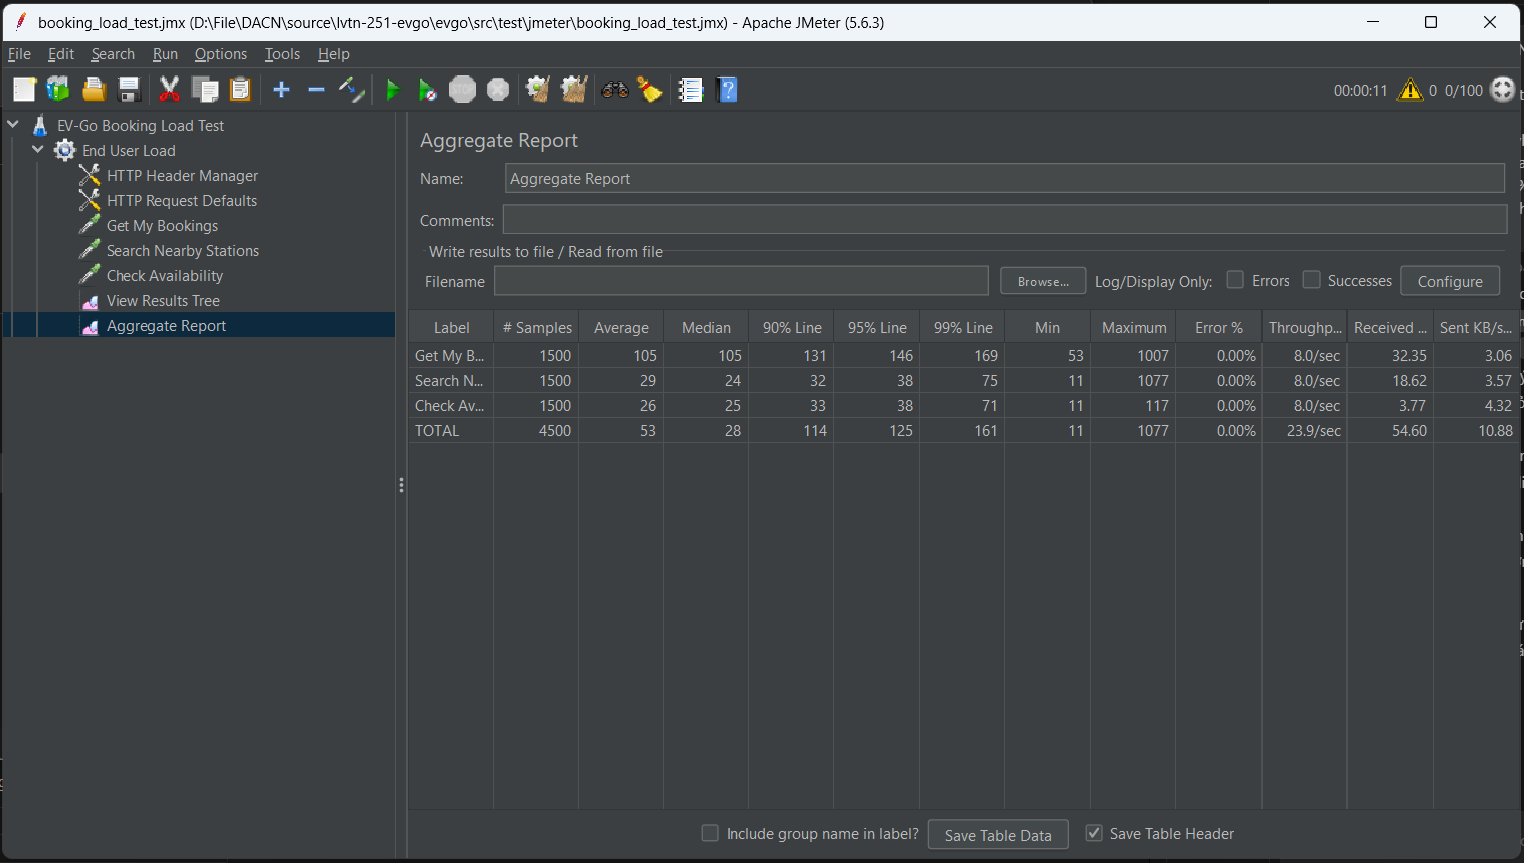
\includegraphics[width=\textwidth]{figures/test/jmeter-report.png}
    \caption{Kết quả kiểm thử hiệu năng với công cụ Apache JMeter}
    \label{fig:jmeter_report}
\end{figure}

\subsubsection{Phân tích chỉ số kỹ thuật}
Kết quả thu được (Hình~\ref{fig:jmeter_report}) chứng minh năng lực xử lý vượt
trội của cấu trúc Modular Monolith:

\begin{itemize}
    \item \textbf{Tỷ lệ lỗi:} 0.00\%. Với 4500 mẫu, hệ thống không
          đánh rơi bất kỳ yêu cầu nào, khẳng định độ ổn định tuyệt đối ở tải mục tiêu.
    \item \textbf{Thời gian phản hồi:} Thời gian phản hồi trung bình
          đạt \textbf{53ms}. Chỉ số \textbf{99\% Line}
          chỉ ở mức \textbf{161ms}, nghĩa là 99\% người dùng nhận phản hồi dưới 0.2s.
    \item \textbf{Thông lượng:} Đạt \textbf{23.9 requests/sec}
          (có tính đến thời gian suy nghĩ của người dùng). Hệ thống giải quyết tốt rào cản cổ chai.
\end{itemize}

\subsubsection{Hành trình tối ưu hóa hệ thống}
\hspace*{\parindent}
Trong giai đoạn đầu, khi số lượng CCU vượt 50, hệ thống EVGo từng gặp hiện tượng
nghẽn mạng, latency lên đến 60s và bắt đầu xuất hiện lỗi Timeout.
Qua phân tích, nhóm đã thực hiện 3 cải tiến then chốt:

\begin{enumerate}
    \item \textbf{Tối ưu hóa Database Indexing:} Đánh Index bổ sung trên
          \texttt{status}, \texttt{station\_id}, \texttt{port\_id}, giúp truy vấn
          chuyển từ quét tuần tự $O(N)$ sang $O(\log N)$.
    \item \textbf{Cấu hình lại HikariCP Connection Pool:} Tái cấu hình
          \texttt{maximum-pool-size} và\\
          \texttt{idle-timeout} để duy trì luồng kết
          nối database khỏe mạnh thay vì phải tạo mới liên tục.
    \item \textbf{Khắc phục N+1 Query:} Cập nhật các Entity Graph và cấu hình
          Hibernate để fetch liên kết dữ liệu trong một câu lệnh JOIN duy nhất,
          thay vì lặp qua từng phần tử.
\end{enumerate}
Những giải pháp này đã giúp hệ thống khôi phục trạng thái hoạt động chớp nhoáng
với độ trễ dưới 200ms như báo cáo cuối cùng.

% ------------------------------------------------------------
\subsection{Đánh giá hệ thống}
% ------------------------------------------------------------

\subsubsection{Đánh giá chức năng}
\hspace*{\parindent}
Bảng~\ref{tab:func_eval} đối chiếu từng nhóm yêu cầu chức năng cốt lõi với mức độ
hoàn thành thực tế của hệ thống EV-Go. Trong tổng số 8 nhóm yêu cầu, hệ thống
hoàn thành đầy đủ 4 nhóm và hoàn thành một phần 4 nhóm còn lại do các giới hạn
về nguồn lực và môi trường triển khai.

\begin{center}
    \renewcommand{\arraystretch}{1.5}
    \begin{longtable}{|>{\raggedright\arraybackslash}m{0.28\textwidth}|>{\centering\arraybackslash}m{0.22\textwidth}|>{\raggedright\arraybackslash}m{0.36\textwidth}|}
        \caption{Ma trận đánh giá hoàn thành yêu cầu chức năng}
        \label{tab:func_eval} \\
        \hline
        \textbf{Nhóm yêu cầu} & \textbf{Trạng thái} & \textbf{Ghi chú} \\
        \hline
        \endfirsthead
        
        \hline
        \textbf{Nhóm yêu cầu} & \textbf{Trạng thái} & \textbf{Ghi chú} \\
        \hline
        \endhead
        
        Quản lý người dùng \& Xác thực & Hoàn thành một phần & Đăng ký và đăng nhập bằng email hoạt động đầy đủ. Luồng đăng nhập qua Google chưa hoạt động được do gặp vấn đề trong quá trình tích hợp. \\
        \hline
        Bản đồ \& Tìm kiếm trạm sạc & Hoàn thành & Tích hợp Map API, bộ lọc theo loại trụ sạc và trạng thái cổng. \\
        \hline
        Đặt chỗ (Booking) & Hoàn thành & Redis Distributed Lock, phát hiện xung đột thời gian thực, tự hủy đặt chỗ quá hạn. \\
        \hline
        Điều khiển sạc (Charging) & Hoàn thành & Giao tiếp OCPP 1.6J và truyền dữ liệu thời gian thực qua SSE. Đã kiểm thử trên môi trường mô phỏng; chưa kiểm thử với trụ sạc vật lý. \\
        \hline
        Thanh toán \& Hóa đơn & Hoàn thành một phần & ZaloPay Deep link và Webhook hoạt động trên Sandbox. Luồng tự động hoàn tiền chưa hoàn thiện. \\
        \hline
        Quản trị trạm (Web Admin) & Hoàn thành một phần & Quản lý dữ liệu và cài đặt cơ bản hoàn chỉnh. Biểu đồ doanh thu và báo cáo tài chính chuyên sâu chưa được tích hợp. \\
        \hline
        Thông báo đẩy (Push Notification) & Hoàn thành & Thông báo thời gian thực qua Expo Push API được tích hợp hoàn chỉnh. \\
        \hline
        Đánh giá \& Phản hồi (Review) & Hoàn thành một phần & Người dùng có thể gửi đánh giá; luồng báo cáo và phản hồi từ chủ trạm chưa hoàn thiện. \\
        \hline
    \end{longtable}
\end{center}

\subsubsection{Đánh giá phi chức năng và kiến trúc}
\begin{itemize}
    \item \textbf{Hiệu năng:} Đáp ứng lượng truy cập đồng thời lớn với độ trễ thấp, sẵn sàng cho việc mở rộng tải trọng khi triển khai thực tế. Dù vậy, khả năng chịu lỗi của hệ thống đối với các sự cố phần cứng (điển hình như luồng xử lý ngoại lệ khi trạm sạc mất kết nối mạng đột ngột) vẫn chưa tự động phục hồi hoàn toàn và cần sự can thiệp thủ công.
    \item \textbf{Bảo mật:} Hệ thống triển khai nhiều lớp bảo vệ độc lập:
        \begin{itemize}
            \item \textbf{Xác thực phiên:} Sử dụng JWT (JSON Web Token) với thời gian sống có giới hạn, kết hợp cơ chế Refresh Token để duy trì phiên đăng nhập an toàn.
            \item \textbf{Phân quyền:} Áp dụng Role-Based Access Control (RBAC), phân tách rõ quyền hạn giữa người dùng cuối, chủ trạm và quản trị viên hệ thống.
            \item \textbf{Tích hợp thanh toán:} Mọi callback từ ZaloPay đều được xác thực chữ ký HMAC-SHA256 trước khi xử lý, ngăn chặn hiệu quả các yêu cầu giả mạo.
            \item \textbf{Bảo mật kênh truyền:} Toàn bộ giao tiếp giữa ứng dụng di động và Backend sử dụng HTTPS; kết nối WebSocket với trụ sạc sử dụng WSS khi triển khai trên môi trường production.
        \end{itemize}
    \item \textbf{Kiến trúc:} Áp dụng triệt để kiến trúc Modular Monolith với Spring Modulith kết hợp kiến trúc hướng sự kiện, hệ thống duy trì được tính độc lập giữa các module. Việc ngăn chặn phụ thuộc vòng tại thời điểm biên dịch giúp tối ưu hóa quá trình phát triển độc lập và tạo nền tảng vững chắc để chuyển đổi các module tải cao (như phân hệ WebSocket/SSE) thành Microservices trong tương lai.
\end{itemize}

\subsubsection{Đánh giá giao diện và trải nghiệm người dùng (UI/UX)}
\begin{itemize}
    \item \textbf{Tính thẩm mỹ:} Giao diện ứng dụng di động đa nền tảng (React Native Expo) áp dụng phong cách thiết kế hiện đại, sử dụng Tailwind để đồng bộ hệ thống màu sắc. Kết hợp giao diện tối màu giúp tăng tính thẩm mỹ và thân thiện với thị giác người dùng.
    \item \textbf{Tính khả dụng:} Luồng thao tác của người dùng được sắp xếp logic. Các màn hình chính được bố trí trực quan, sử dụng các hiệu ứng tải trang và hệ thống thông báo theo thời gian thực (Push Notification, SSE) để tăng khả năng phản hồi trực tiếp với người dùng và xử lý mượt mà các trạng thái của dòng dữ liệu.
\end{itemize}

\newpage
\section{Kết luận}

\subsection{Kết quả đạt được}
Sau quá trình nghiên cứu và thực hiện đồ án, nhóm đã xây dựng thành công hệ thống quản lý trạm sạc xe máy điện EVGo với các kết quả cụ thể như sau:

\begin{itemize}
    \item \textbf{Về mặt chức năng:}
    \begin{itemize}
        \item Hoàn thiện các luồng nghiệp vụ cơ bản cho ba đối tượng người dùng: Người dùng (User), Quản trị viên (Super Admin) và Chủ trạm (Station Owner).
        \item Tích hợp thành công tính năng đăng nhập nhanh (SSO) thông qua Google cho các tài khoản thuộc tổ chức \texttt{hcmut.edu.vn}.
        \item Xây dựng quy trình đăng ký và xét duyệt chủ trạm trực tuyến, bao gồm cơ chế gửi email xác thực tự động.
    \end{itemize}
    
    \item \textbf{Về mặt kỹ thuật và giao diện:}
    \begin{itemize}
        \item Áp dụng thành công kiến trúc Modular Monolith, giúp hệ thống dễ dàng bảo trì và mở rộng.
        \item Giao diện người dùng được thiết kế hiện đại với chế độ Dark Mode mặc định, đảm bảo tính thẩm mỹ và trải nghiệm người dùng tốt.
    \end{itemize}
\end{itemize}

\subsection{Hạn chế}
Bên cạnh những kết quả đạt được, hệ thống vẫn còn tồn tại một số hạn chế nhất định:

\begin{itemize}
    \item \textbf{Phạm vi người dùng:} Tính năng đăng nhập nhanh (SSO) hiện tại chỉ giới hạn cho các email thuộc tổ chức \texttt{hcmut.edu.vn} do các rào cản về chi phí khi mở rộng phạm vi xác thực cho người dùng phổ thông.
    \item \textbf{Kết nối phần cứng:} Hệ thống chưa được kết nối với các trạm sạc vật lý thực tế. Việc giao tiếp hiện tại hoàn toàn dựa trên cơ chế giả lập thông qua giao thức OCPP, do đó chưa thể đánh giá được toàn diện các vấn đề phát sinh trong môi trường vận hành thực tế với phần cứng.
\end{itemize}

\subsection{Hướng phát triển}
Dựa trên những kết quả và hạn chế đã phân tích, nhóm đề xuất các hướng phát triển trong tương lai để hoàn thiện hệ thống:

\begin{itemize}
    \item \textbf{Tích hợp Trí tuệ nhân tạo (AI):} Nghiên cứu và áp dụng các thuật toán AI để cung cấp tính năng gợi ý trạm sạc tối ưu dựa trên vị trí và thói quen của người dùng, cũng như dự đoán nhu cầu sạc tại các khu vực khác nhau để hỗ trợ chủ trạm trong việc vận hành.
    \item \textbf{Mở rộng phạm vi xác thực:} Tìm kiếm các giải pháp tối ưu chi phí để mở rộng tính năng SSO cho các tài khoản Google cá nhân và các nền tảng mạng xã hội khác, giúp hệ thống tiếp cận được nhiều người dùng hơn.
    \item \textbf{Tối ưu hóa công cụ quản trị:} Tiếp tục phát triển và hoàn thiện nền tảng Website dành cho các đối tượng quản lý (Super Admin, Station Owner, Staff), tập trung vào các công cụ báo cáo, thống kê chuyên sâu thay vì phát triển ứng dụng di động riêng cho nhóm đối tượng này.
\end{itemize}
% ===== References =====
\newpage
\nocite{*}  
\bibliographystyle{plain}
\bibliography{references}
\end{document}